
\newcommand{\fCII} {\emath{f^{C \times 2}}}
\newcommand{\fPII} {\emath{f^{P \times 2}}}
\section{Experimental Results on Synthetic Data}\label{sec:synData}
\subsection{Synthetic Scalar and Gradient Data}
\label{section:synthetic}

To measure the quality of our reconstruction,
we used a number of synthetic scalar and gradient data sets.
Given a point $p$,
let $f^{L_1}_{p}(q)$ be the $L_1$ distance from $p$ to $q$.
A Cube data set is generated by sampling $f^{L_1}_p$
and its gradients on vertices of the regular grid.

Level sets of $f^{L_1}_p$ are cubes whose edges are
parallel to the coordinate axes
and whose facets are orthogonal to those axes.
By rotating $f^{L_1}_p$ around $p$, 
we can generate a scalar field whose level sets are cubes
that are not axis-aligned.
By taking the minimum of two (rotated) scalar fields, 
$f^{L_1}_p$ and $f^{L_1}_{p'}$, 
centered around two different points, $p$ and $p$', respectively,
we get a scalar field whose level sets are the boundaries
of the unions of the two cubes.
We call such data sets TwoCubes and use them 
with various rotations as test sets.

Let $\ell$ be a line.
Let $f^C_{\ell}(q)$ be the Euclidean distance from point $q$ to $\ell$.
The level sets of $f^C_{\ell}(q)$ are infinite cylinders around $\ell$.
Let $\fCII_{\ell,r}(q)$ equal $|f^C_{\ell}(q) - r|$.
The level sets of $\fCII_{\ell,r}(q)$  are pairs of infinite cylinders
at equal distances from the cylinder of radius $r$ around $\ell$.
Let $\fPII_{p,\ell}(q)$ be the distance from $q$ to the plane 
that contains point $p$ and is orthogonal to $\ell$.
Let $f^A_{p,\ell,r}(q)$ be the maximum 
of $\fCII_{\ell,r}(q)$ and of $\fPII_{p,\ell}(q)$.
The level sets are the boundaries of thickened annuli.

The width of the thickened annuli defined by $f^A_{p,\ell,r}$
equals their height.
We can adjust change the difference between the width and height
by adding a constant $c$ to $\fCII_{\ell,r}$.
Let $f^A_{p,\ell,r,c}(q)$ be the maximum 
of $\fCII_{\ell,r}(q)+c$ and of $\fPII_{p,\ell}(q)$.
If $c$ is positive, then the height is $c$ units greater than the width.
If $c$ is negative, then the height is $c$ units less than the width.

Define $f^F_{p,\ell,r,c}(q)$ as the minimum
of $f^A_{p,\ell,r,c}(q)$ and $f^A_{p,\ell,r,-c}(q)$.
The level sets of $f^F_{p,\ell,r,c}(q)$ are the boundaries
of the unions of two thickened annuli.
One annuli has height $c$ units greater than its width
while the other has height $c$ units less than its width.
A Flange data set is a regular grid sampling of $f^F_{p,\ell,r,c}(q)$. 
We use the Flange data sets as test sets.

\subsection{Isosurface Reconstruction on Synthetic Data}
We ran SHREC on 40 Flange datasets with different orientations. Figure~\ref{fig:flangeAngle} shows the summary results.
With synthetic gradients, SHREC produced ``NO" degree errors on the 40 test cases.
Figure~\protect\subref*{fig:flangeAngle3} shows the number of CountDegree errors in running SHREC with gradients computed from the scalar volume using RELIGRAD.
Fourteen cases ($35\%$) produced no degree errors. The mean error was 4.5. The maximum error was 22.
Figure~\protect\subref*{fig:flangeAngle1} shows the number of simplices with angle difference greater than 30$^\circ$, 40$^\circ$ and 50$^\circ$ from the original mesh for the 40 test cases. Figure~\protect\subref*{fig:flangeAngle2} shows  the number of simplices versus the angle difference for one particular dataset (id 16). This particular dataset has no CountDegree errors, it has three simplices with surface angle difference greater than 30 degrees from the original and one simplex above 40 degrees. The mesh itself has approximately 133 thousand simplices. 
Figure~\ref{fig:flange1} shows the result on a single dataset. The magnified region shows edges with dihedral angle less than $140^\circ$ in red blended with a subset of the ``non-sharp" edges. 
\begin{figure}[tb]
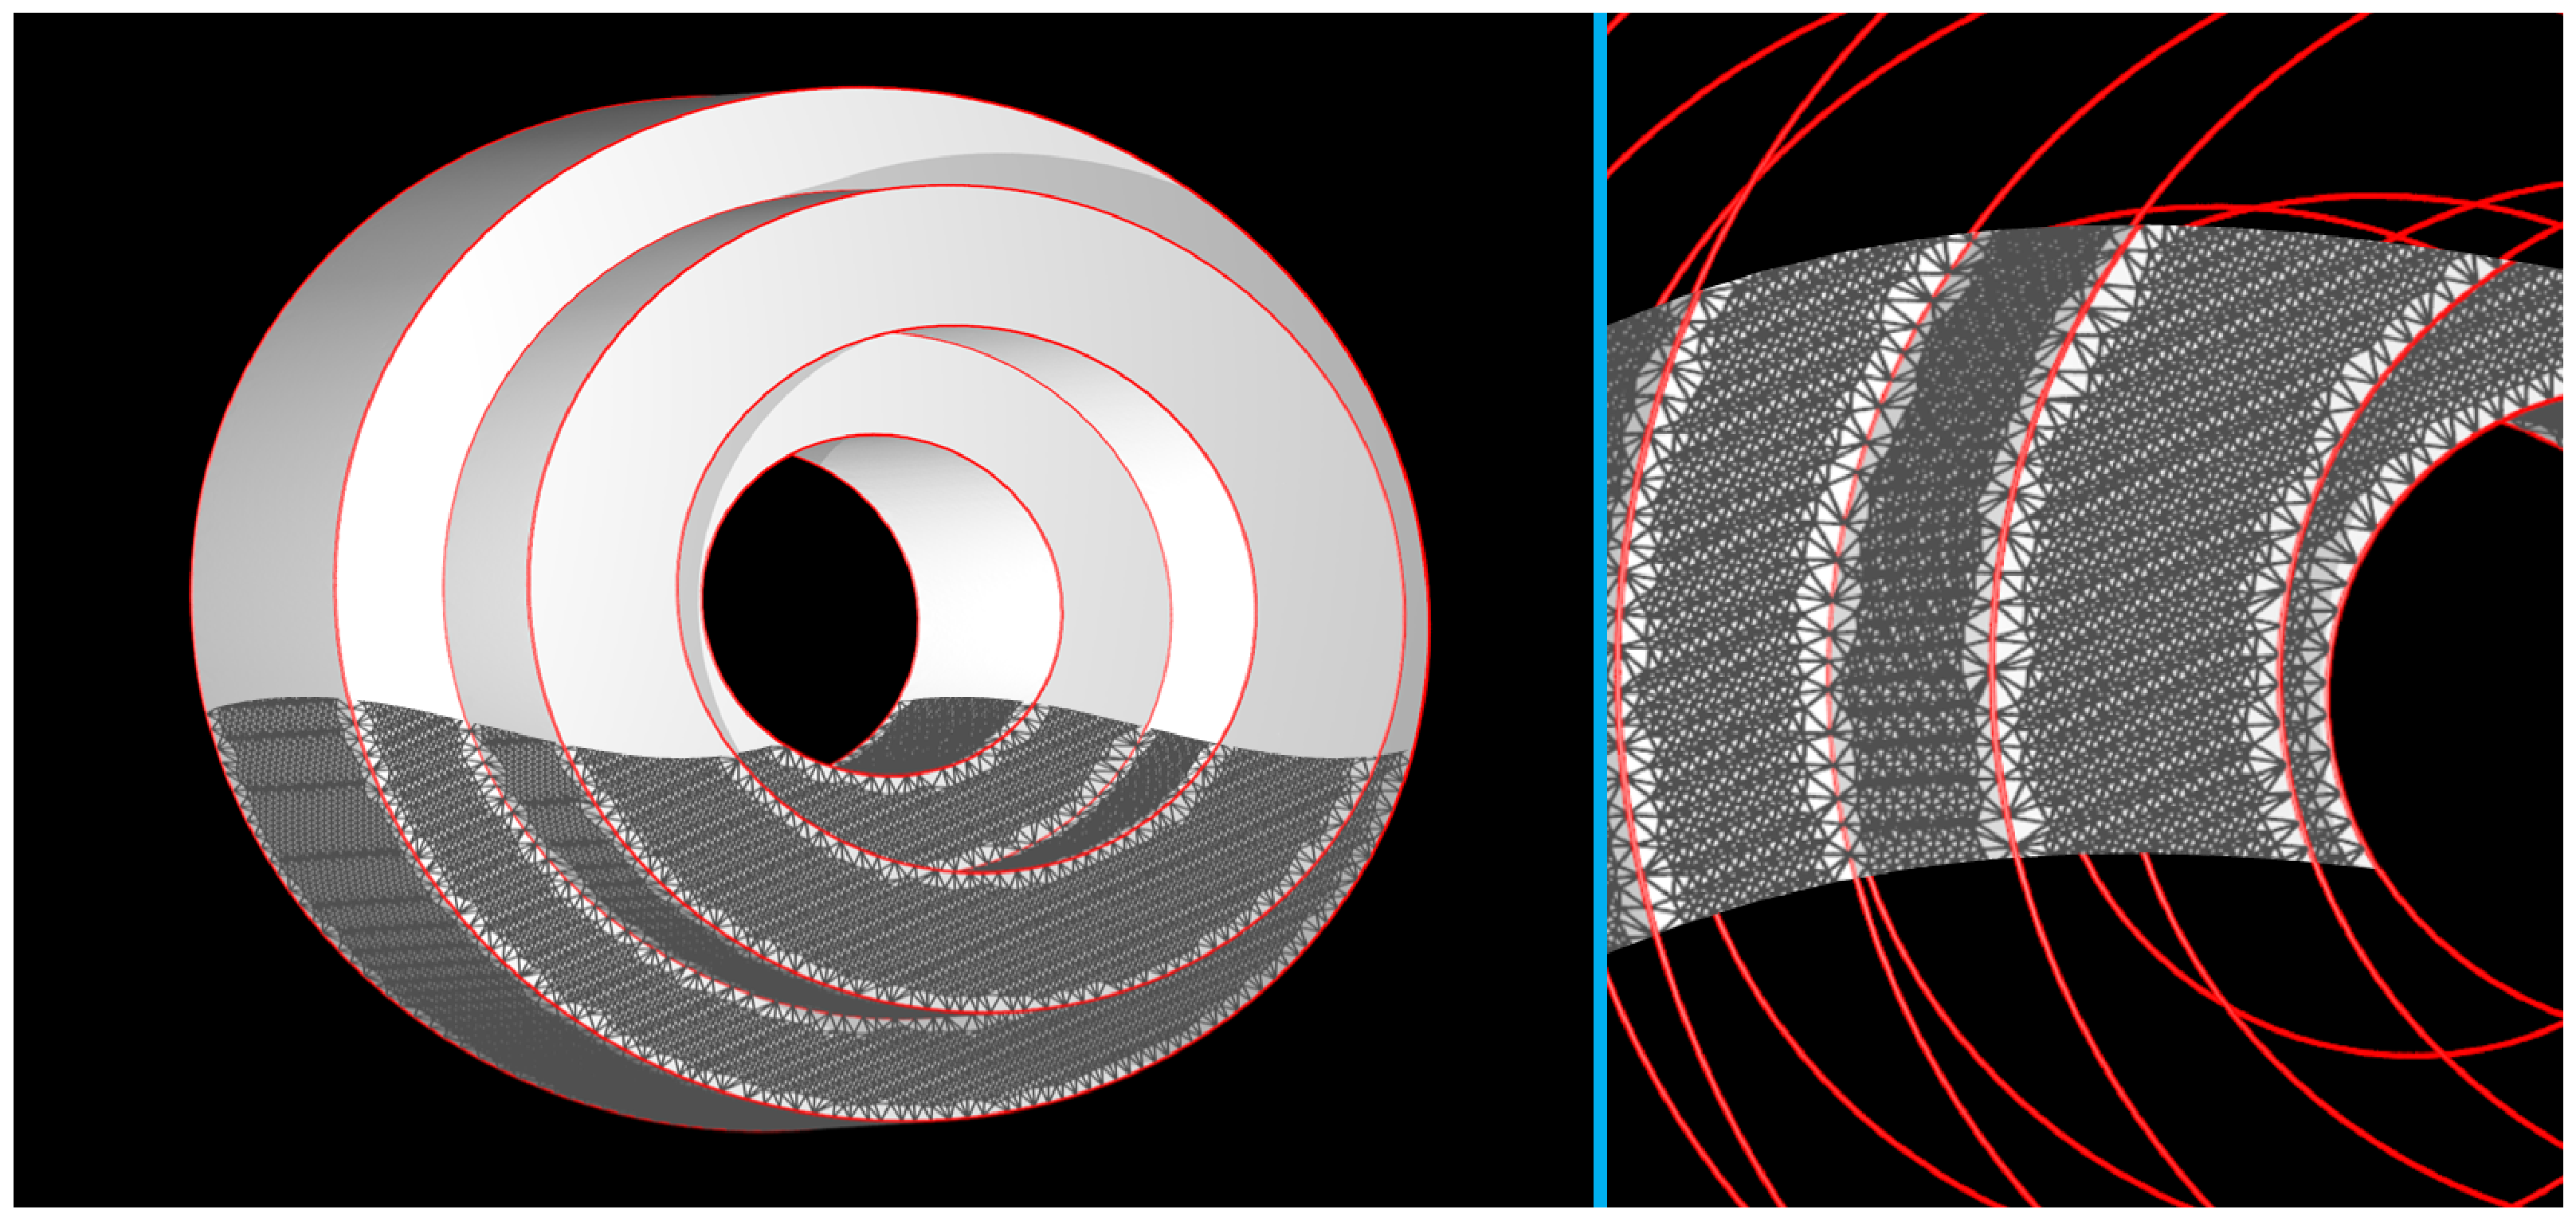
\includegraphics[width=\linewidth]{images/shrecFlangeCombine2.eps}
\caption{Result of SHREC on a Flange dataset. ``Sharp" edges (with dihedral angle less than $140^\circ$) are marked in red. 
``Smooth" edges are in dark grey. The magnified region shows a blend of the ``sharp" edges with a subset of the ``smooth" edges.}
\label{fig:flange1}
\end{figure}
\begin{figure*}[tb]
	\subfloat[]{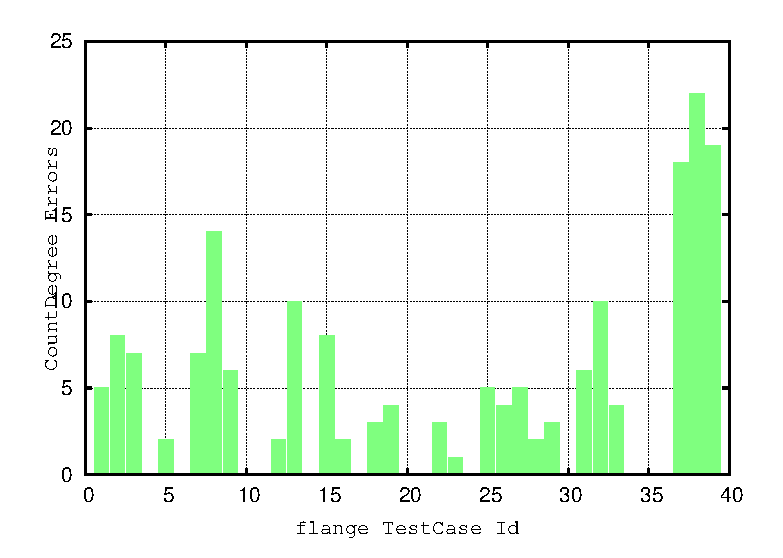
\includegraphics[width=0.33\linewidth]{images/flangeAngle3.eps}\label{fig:flangeAngle3}}
	\subfloat[]{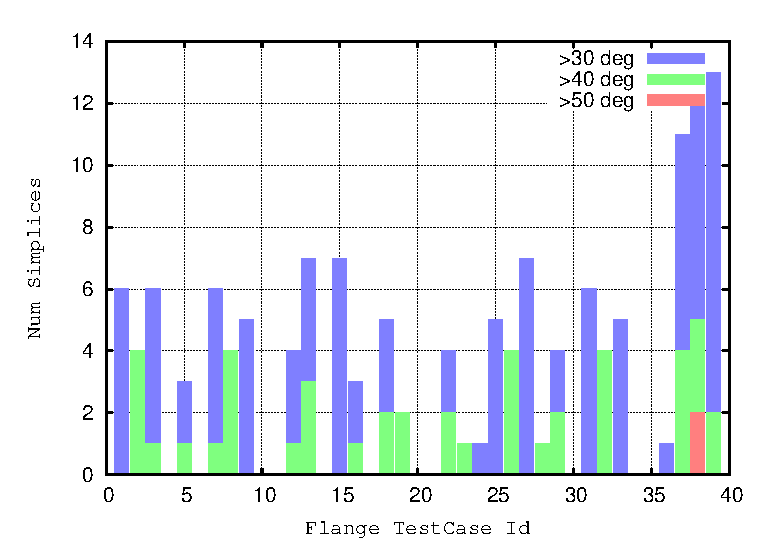
\includegraphics[width=0.33\linewidth]{images/flangeAngle1.eps}\label{fig:flangeAngle1}}
	\subfloat[]{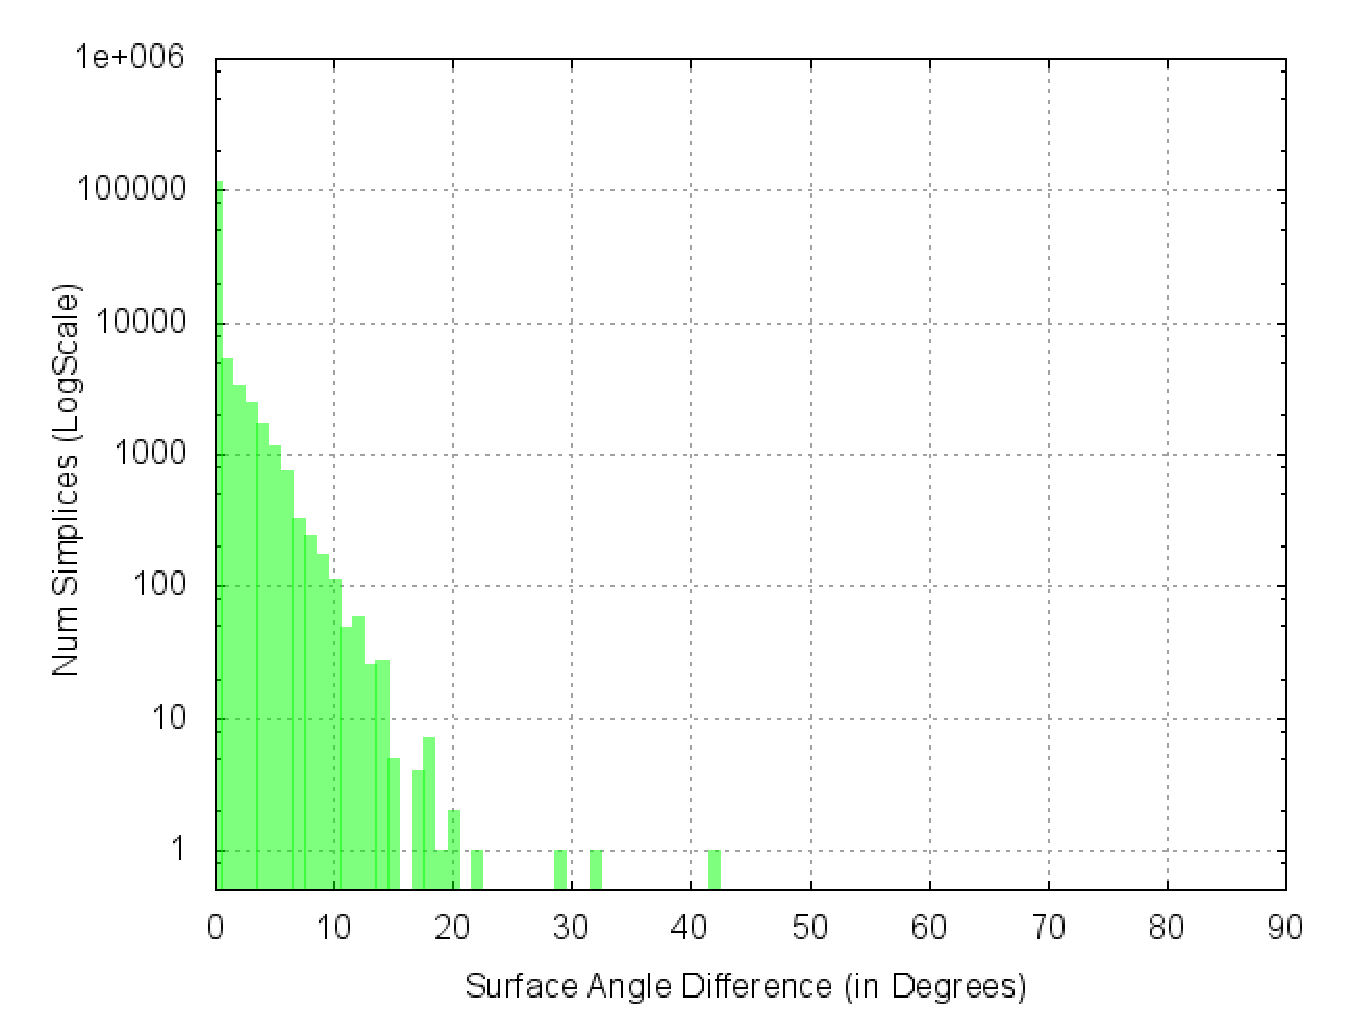
\includegraphics[width=0.33\linewidth]{images/flangeAngle2.eps}\label{fig:flangeAngle2}}
	\caption{SHREC with gradients computed from scalar data using RELIGRAD on 40 datasets. (a) Number of CountDegree errors. (b) Number of simplices with angle difference to ``perfect" mesh above 30, 40 and 50 degrees. (b) Shows the angle distribution of one particular case (16) which has three simplices over 30 degrees and 1 above 40 degrees. Total number of simplices is ~133k.}\label{fig:flangeAngle}
\end{figure*}
\begin{figure*}[tb] 
	\centering
	\subfloat[]{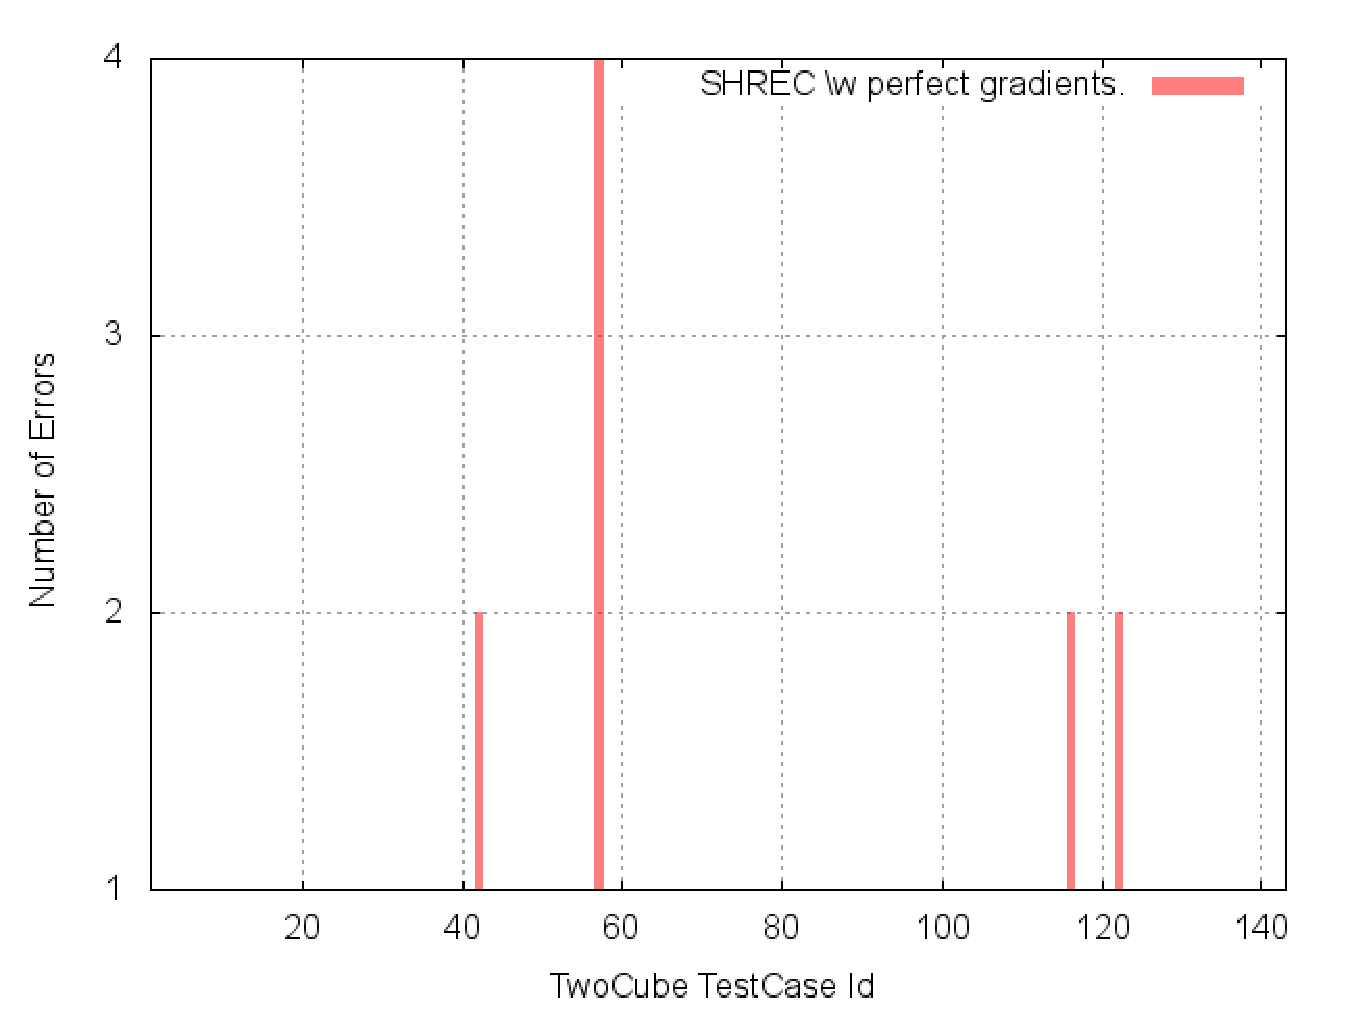
\includegraphics[width=0.3\linewidth]{images/shrecResCol1.eps}\label{fig:shrecTwoCube:a}}
	\subfloat[]{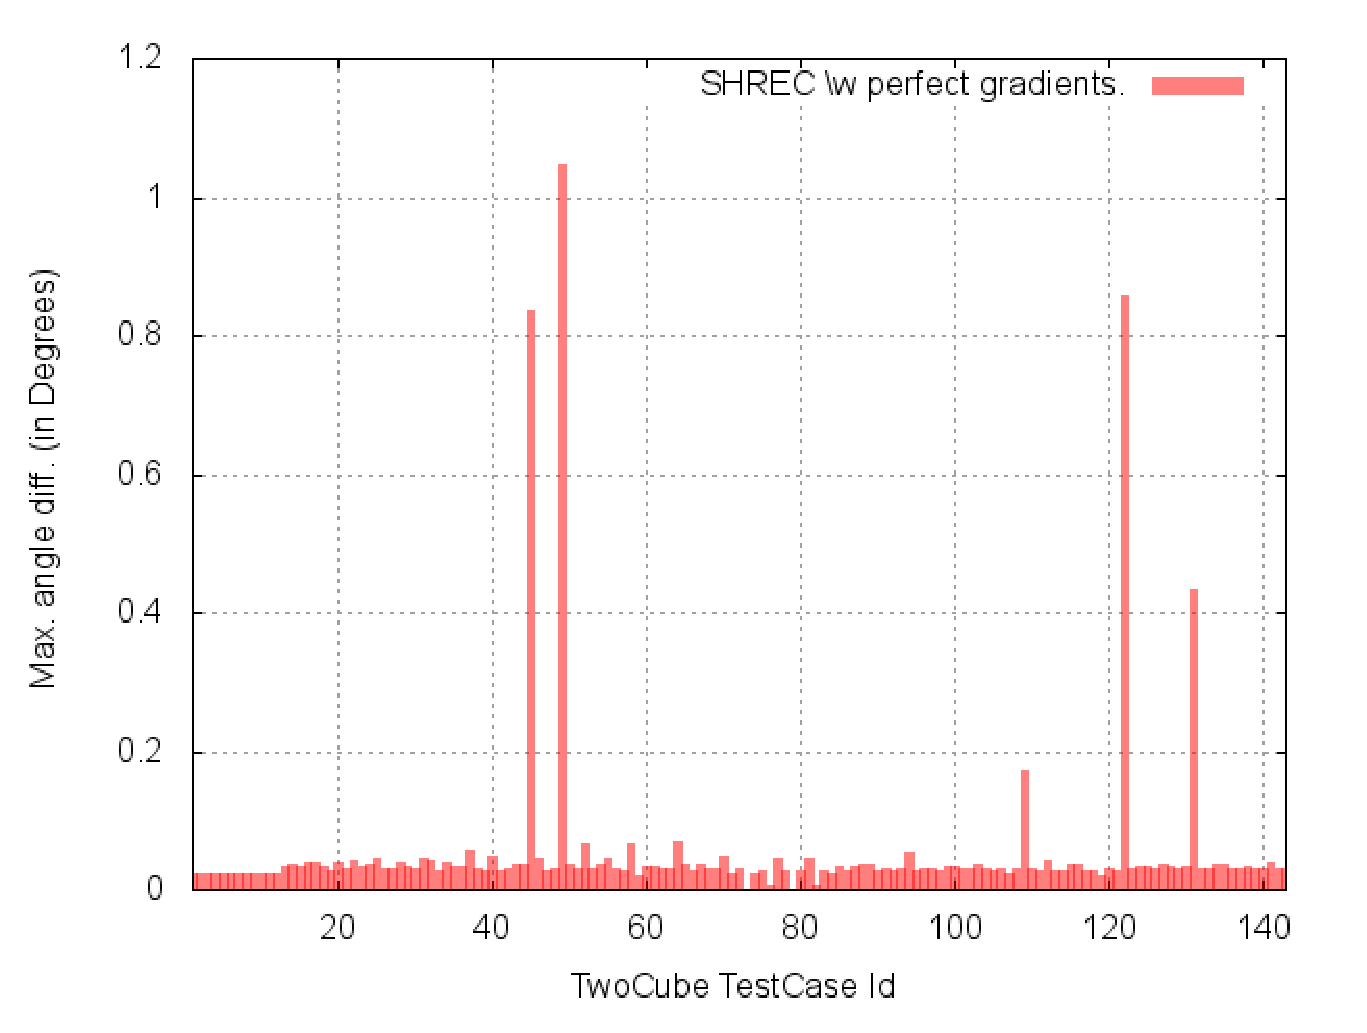
\includegraphics[width=0.3\linewidth]{images/shrecResCol3.eps}\label{fig:shrecTwoCube:b}}\\
	\subfloat[]{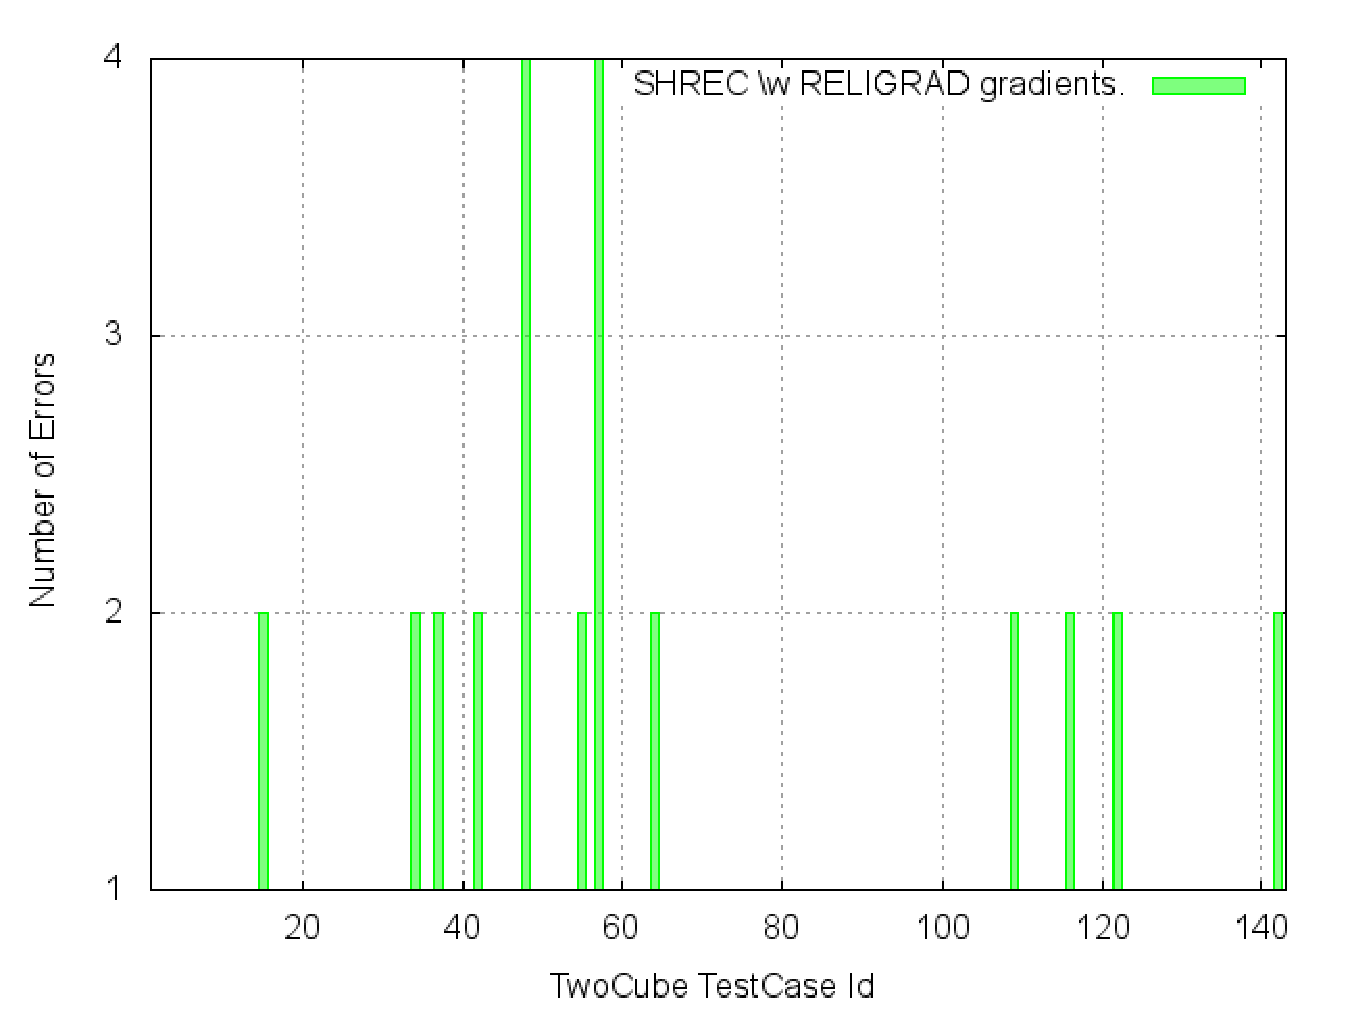
\includegraphics[width=0.3\linewidth]{images/shrecResCol2.eps}\label{fig:shrecTwoCube:c}}
	\subfloat[]{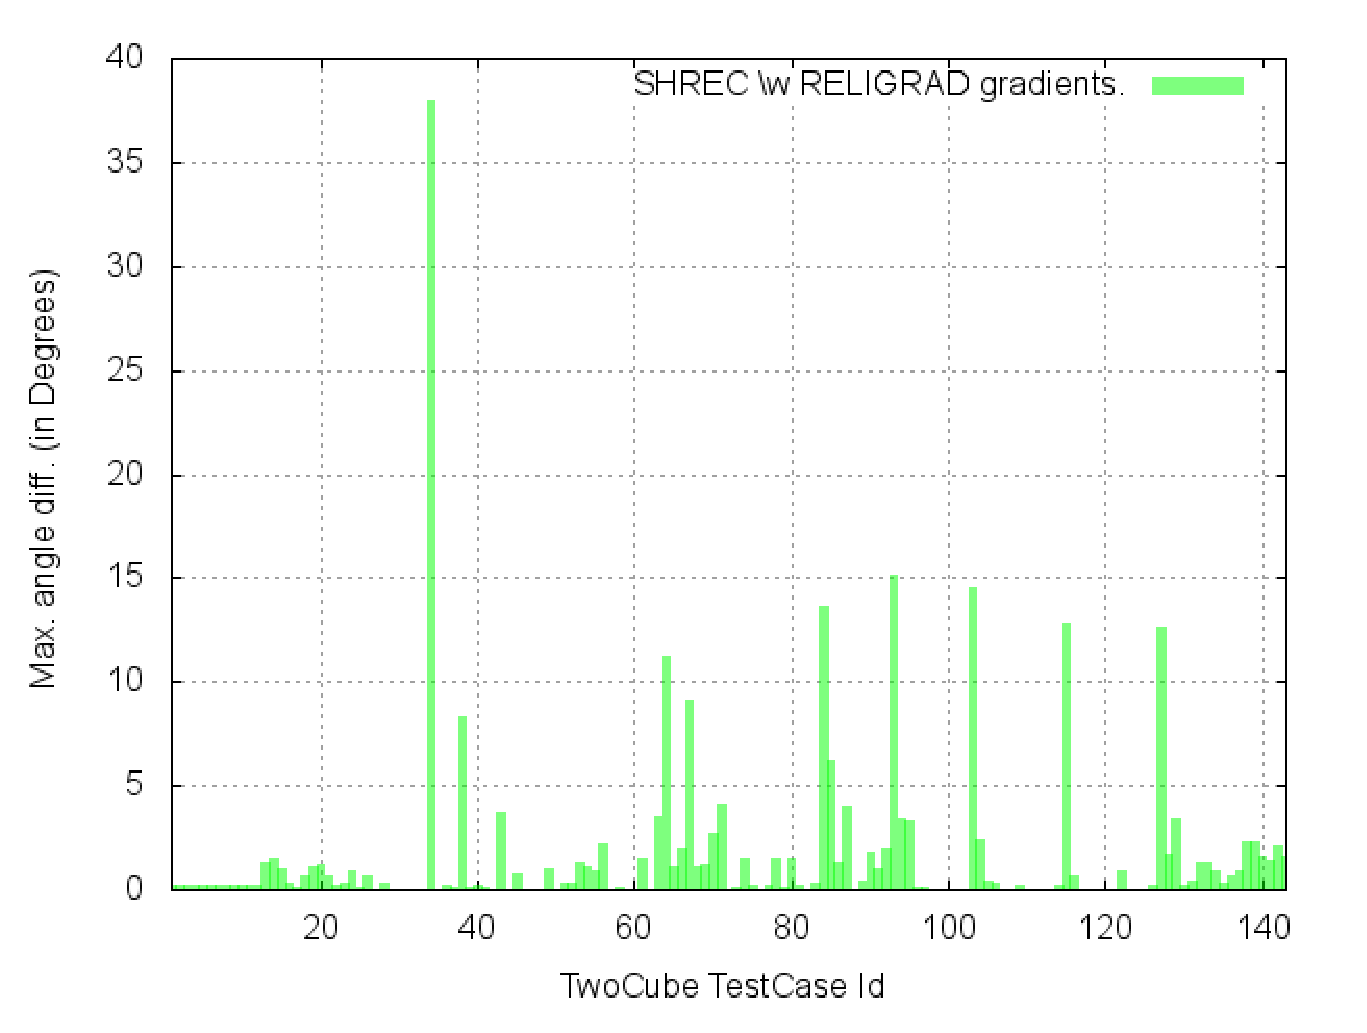
\includegraphics[width=0.3\linewidth]{images/shrecResCol4.eps}\label{fig:shrecTwoCube:d}}
	\caption{SHREC with perfect gradients and with RELIGRAD gradients(computed directly from scalar data.).~\protect\subref{fig:shrecTwoCube:a} shows the number of CountDegree errors when using SHREC along with the correct gradients.~\protect\subref{fig:shrecTwoCube:c} The same result when using gradients computed directly from scalar data (RELIGRAD). ~\protect\subref{fig:shrecTwoCube:b} shows the maximum angle difference from the ``perfect mesh" when using correct gradients.~\protect\subref{fig:shrecTwoCube:d} The same result when using RELIGRAD gradients. }
	\label{fig:shrecTwoCube}
	\vskip-0.2cm
\end{figure*}


We next ran SHREC on 143 TwoCube datasets; Figure~\ref{fig:shrecTwoCube} shows the summary results. As with Flange we first tested SHREC with synthetic gradients and then with gradients computed from the scalar data using RELIGRAD.

Figure~\protect\subref*{fig:shrecTwoCube:a} shows the number of CountDegree errors using the SHREC algorithm along with synthetic gradients at grid vertices as input. Only four test cases have errors, with the maximum having four errors. 
Figure~\protect\subref*{fig:shrecTwoCube:b}, shows the maximum angle difference from the original mesh. The maximum angle difference is 1.05 degrees for the dataset id 50.

Figure~\protect\subref*{fig:shrecTwoCube:c}, shows the CountDegree results using SHREC with RELIGRAD gradients. The maximum number of errors for a single dataset is four. Figure~\protect\subref*{fig:shrecTwoCube:d} shows the maximum angle difference from the original perfect mesh. While the maximum error was 38 degrees for a single test, majority produced very small errors. Figure~\ref{fig:shrecPerfect1} shows the mesh and the edges generated on a particular dataset.

Figure~\protect\subref*{fig:cannon:b},~\protect\subref*{fig:cannon:a} show our results of running SHREC with RELIGRAD on the Cannon datasets. Figure~\protect\subref*{fig:cannon:b} shows the CountDegree errors generated for the 15 cannon sets using gradients computed from RELIGRAD. The maximum error generated was 2. SHREC using synthetic gradients generated 'NO' errors. Figure~\protect\subref*{fig:cannon:a} shows one representative result using SHREC and RELIGRAD directly from scalar data. The magnified region shows a portion of the sharp edge. 

Similarly, Figure ~\protect\subref*{fig:cone:b},~\protect\subref*{fig:cone:a} show our results of running SHREC with RELIGRAD on the Cone datasets.
A single cone data set using synthetic gradients produces two Count Degree errors. With gradients computed from RELIGRAD the maximum number of errors is 4.
\begin{figure}[tb]
	\includegraphics[width=\linewidth]{images/shrecperfect.eps}
	\caption{Result of SHREC on a twoCube dataset. The FindSharp Edges are marked in red. Smooth edges are shown in cyan. The magnified region shows the output mesh edges around a corner.}
	\label{fig:shrecPerfect1}
\end{figure}
\begin{figure}[tb]
	\subfloat[]{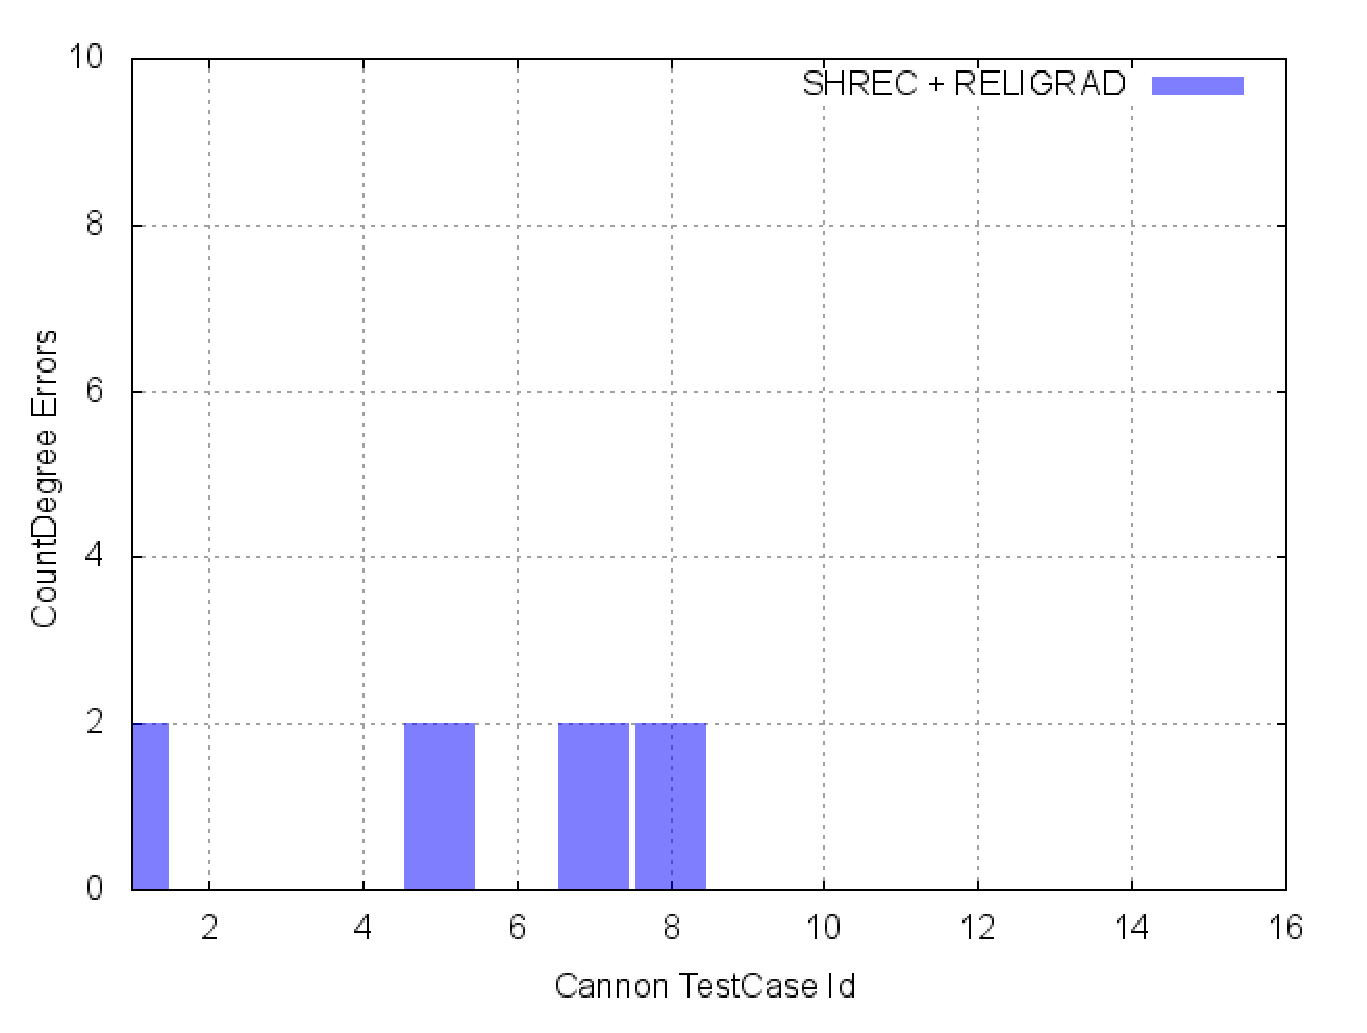
\includegraphics[width=0.5\linewidth]{images/cannon.eps}\label{fig:cannon:b}}
	\subfloat[]{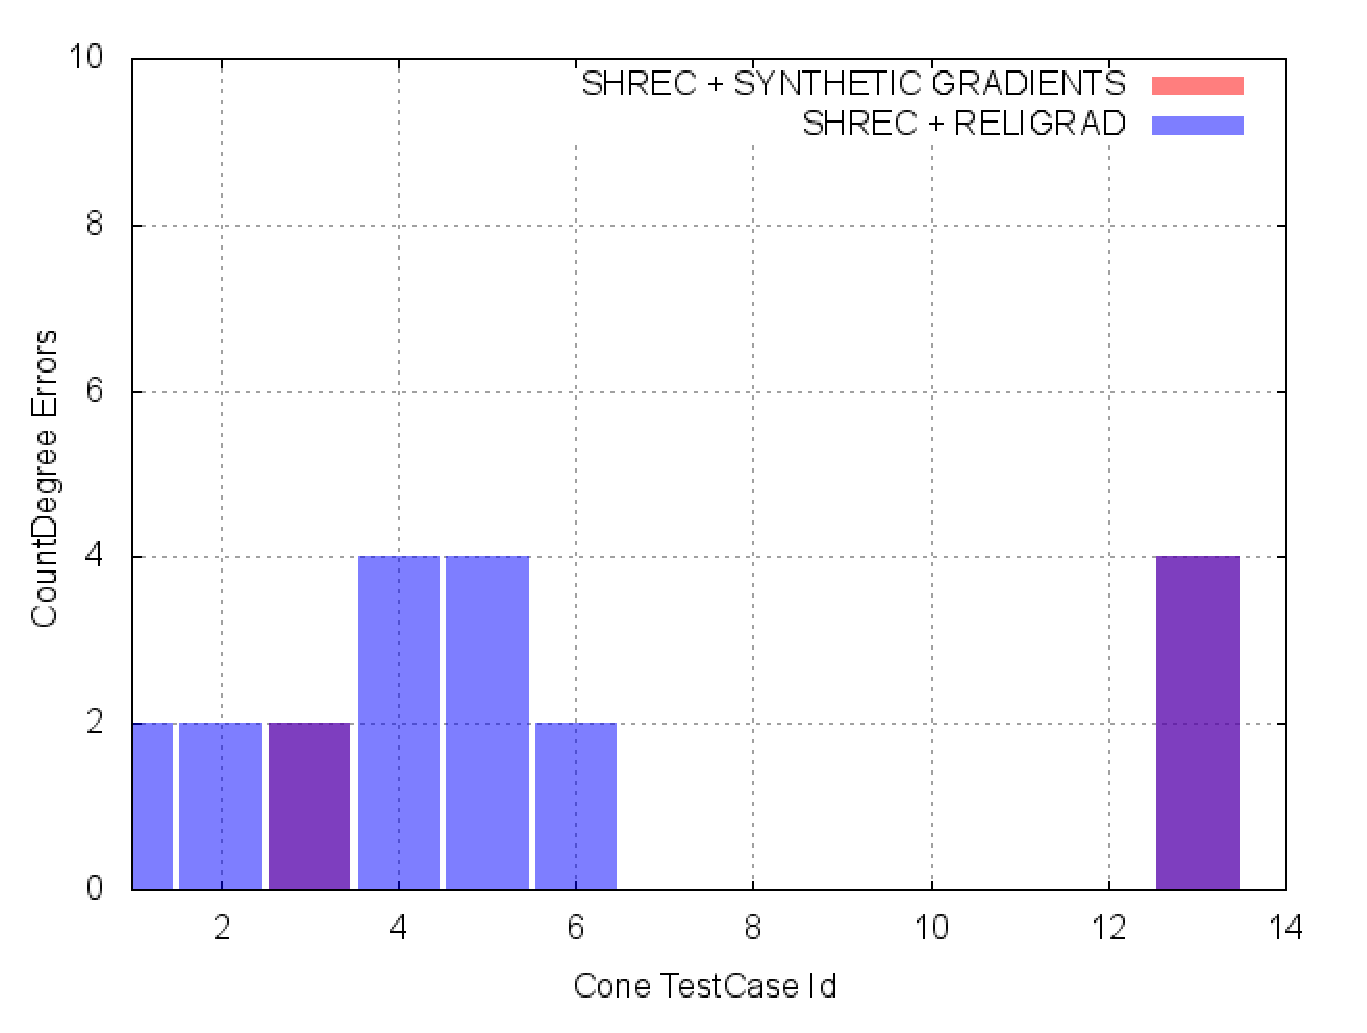
\includegraphics[width=0.5\linewidth]{images/cone.eps}\label{fig:cone:b}}
	\caption{Summary result of algorithm SHREC on Cannon and cone Datasets. (a) CountDegree Errors on 15 Cannon datasets using RELIGRAD gradients. SHREC with perfect gradients had no errors and is not shown. (b) CountDegree errors on 14 Cone datasets using RELIGRAD and perfect gradients.}
	\label{fig:cannon_cone_summary}
\end{figure}
\begin{figure}[tb]
	\subfloat[]{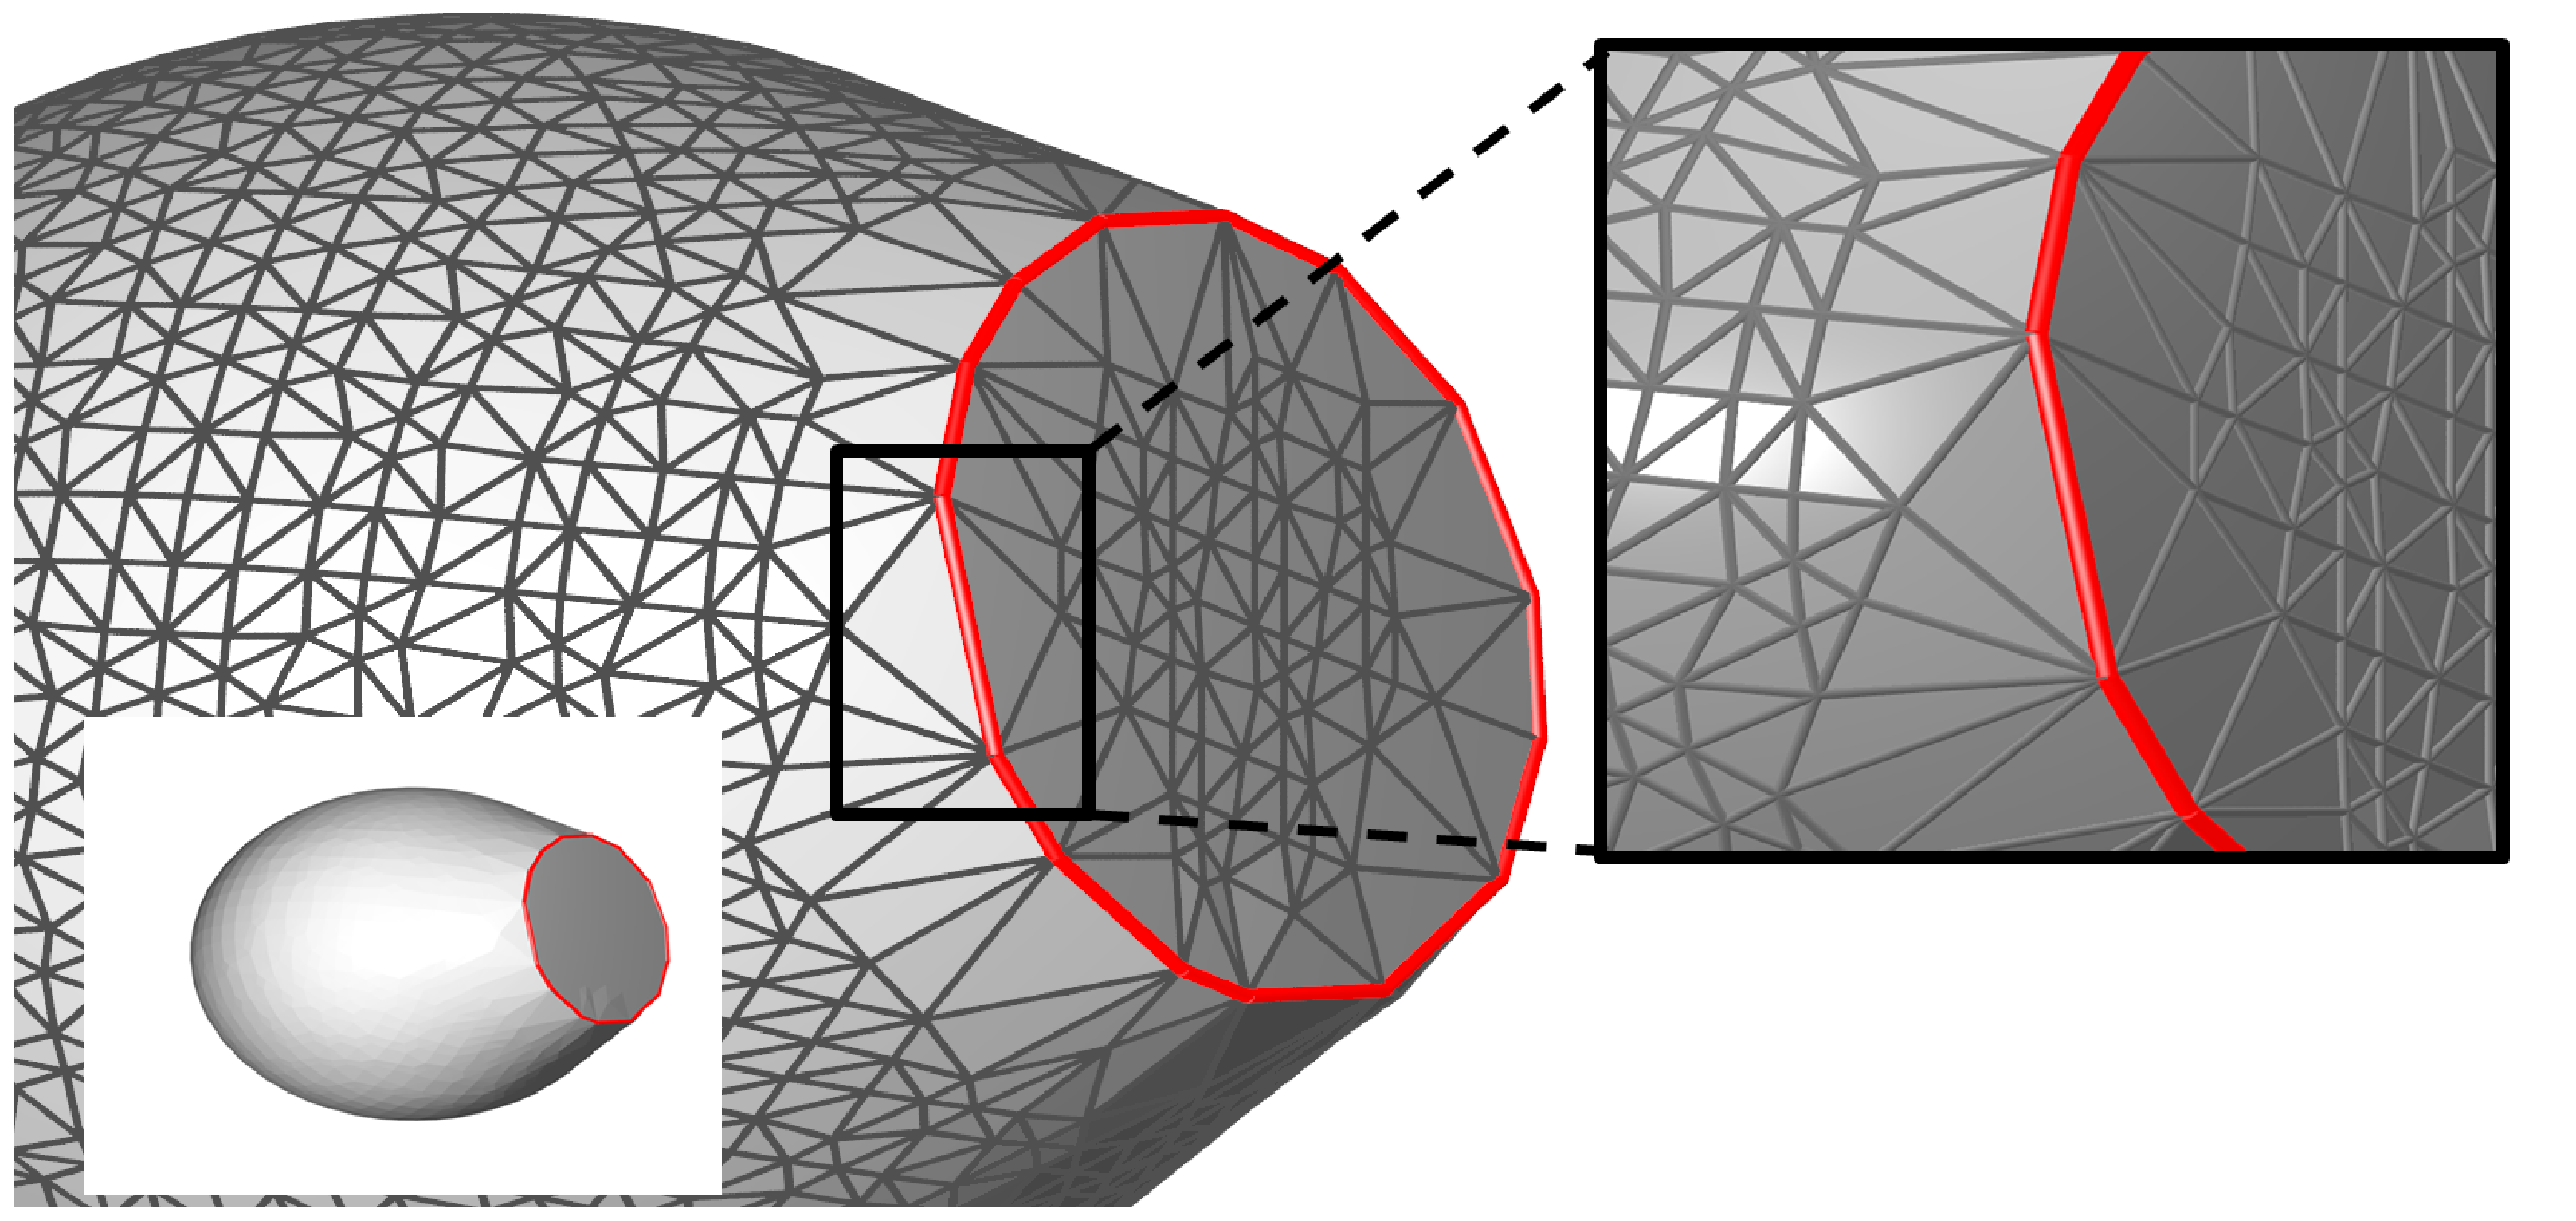
\includegraphics[width=0.5\linewidth]{images/cannon2.eps}\label{fig:cannon:a}}
	\subfloat[]{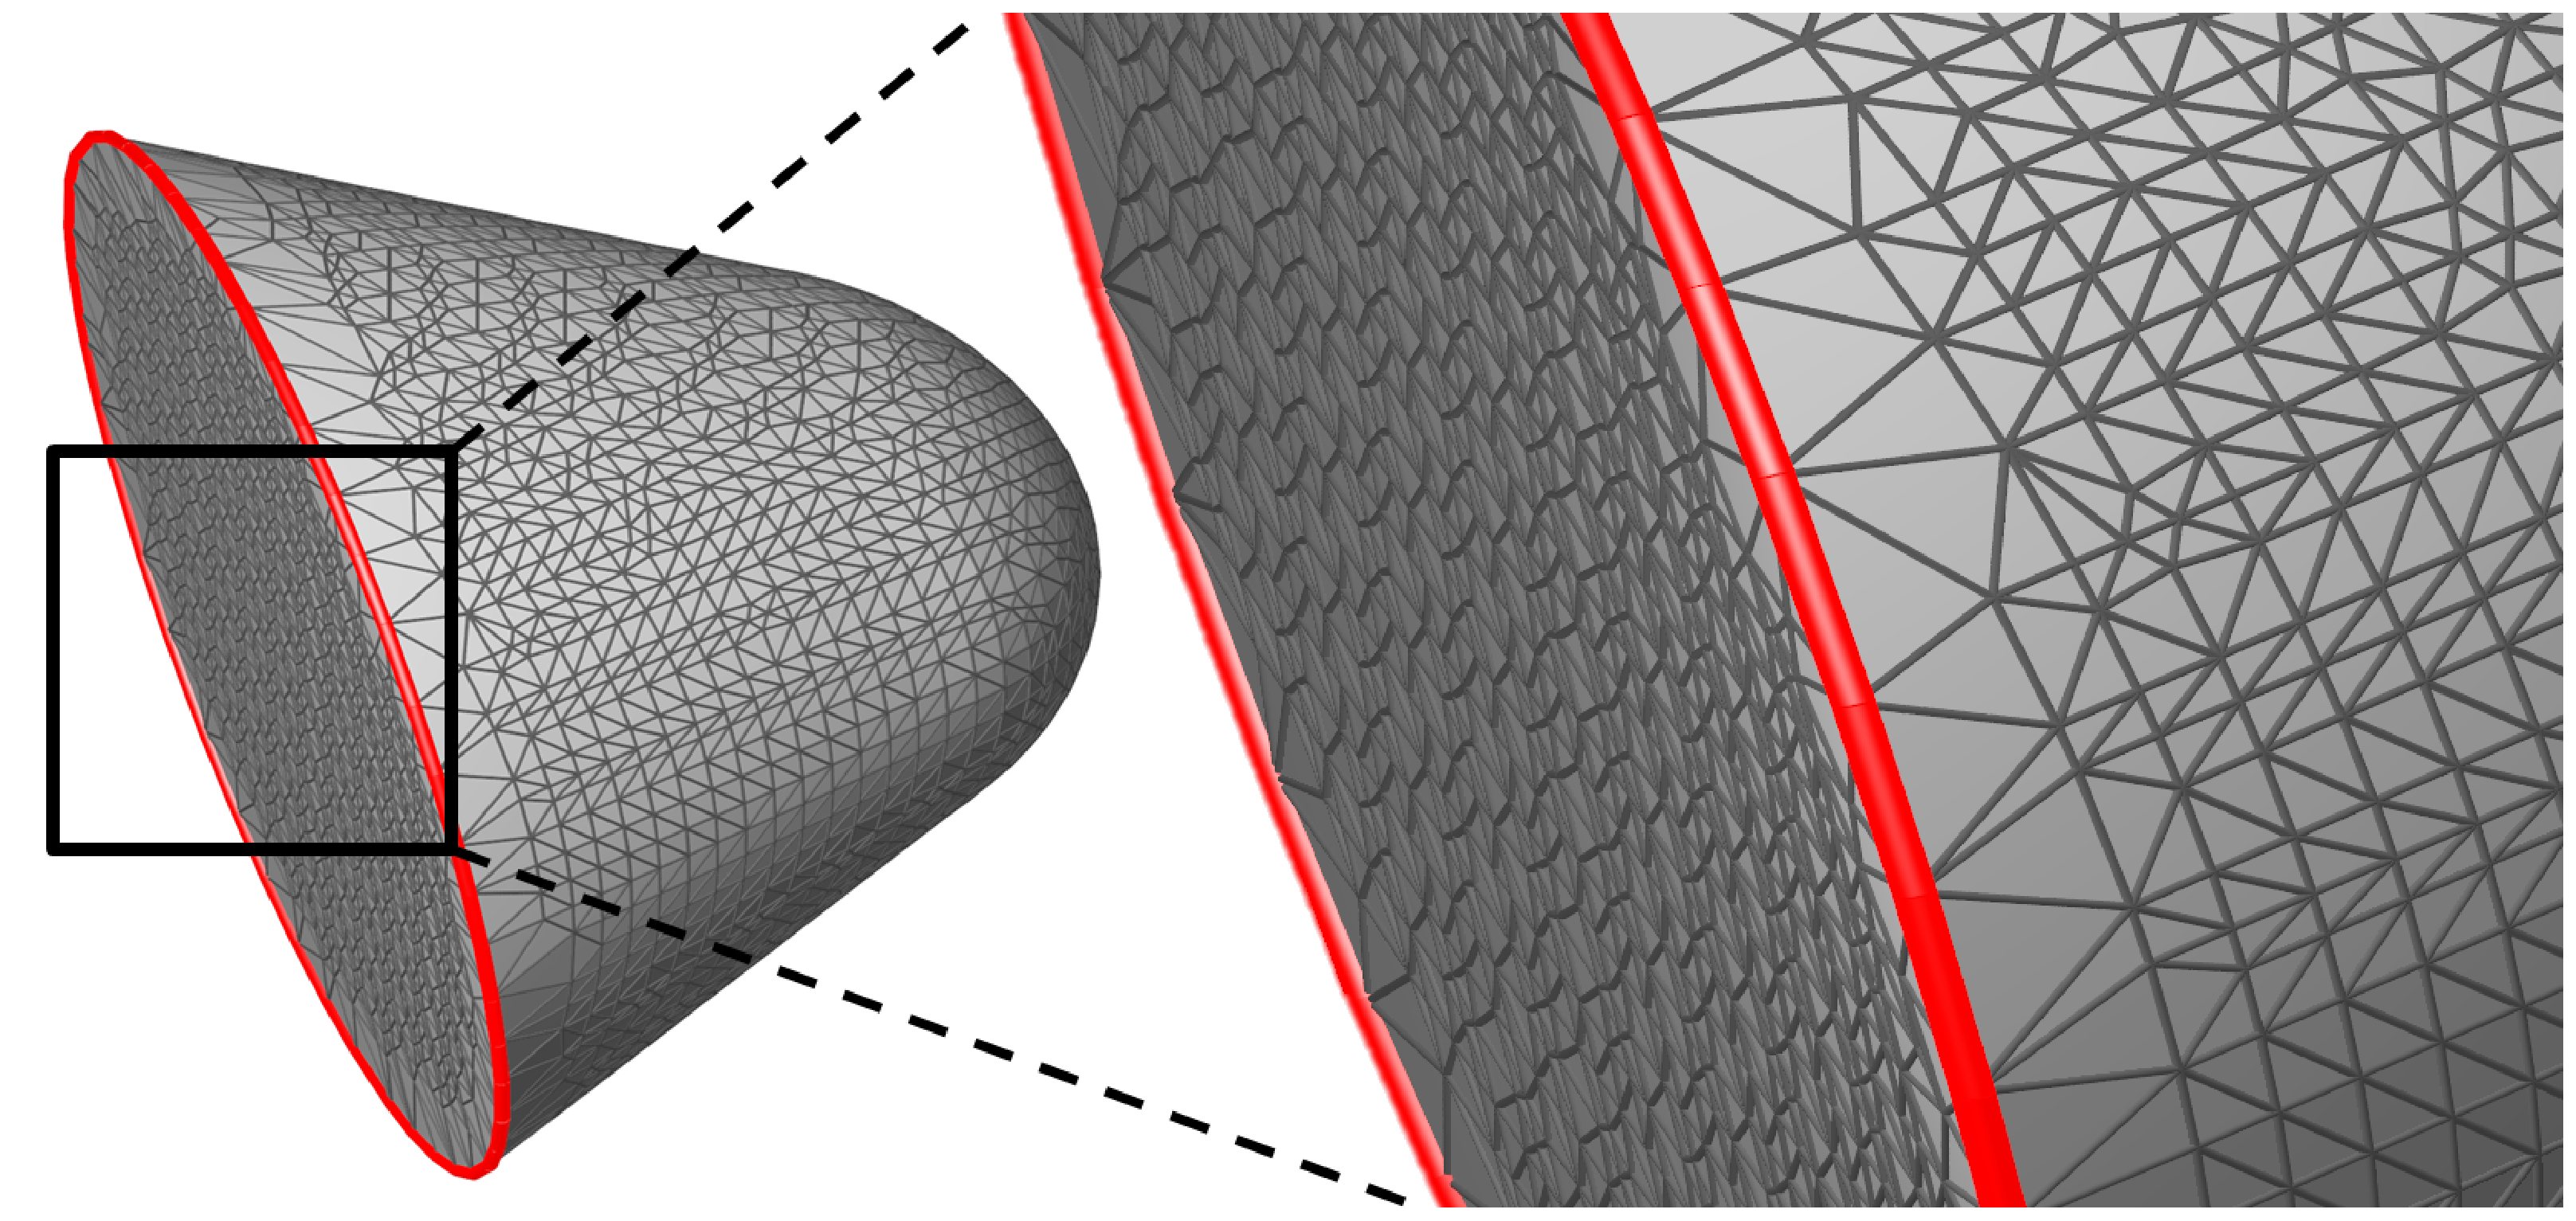
\includegraphics[width=0.5\linewidth]{images/cone2.eps}\label{fig:cone:a}}
	\caption{Result of algorithm SHREC with RELIGRAD gradients on Cannon and Cone datasets}
	\label{fig:cannon_cone}
\end{figure}
\section{Experimental Results on CT Data}

\subsection{Description of CT Data Sets}

\subsection{Comparison with Other Algorithms}
\paragraph{Comparison with MergeSharp}
%#150
\begin{figure}[htb]
	\centering
	\subfloat[]{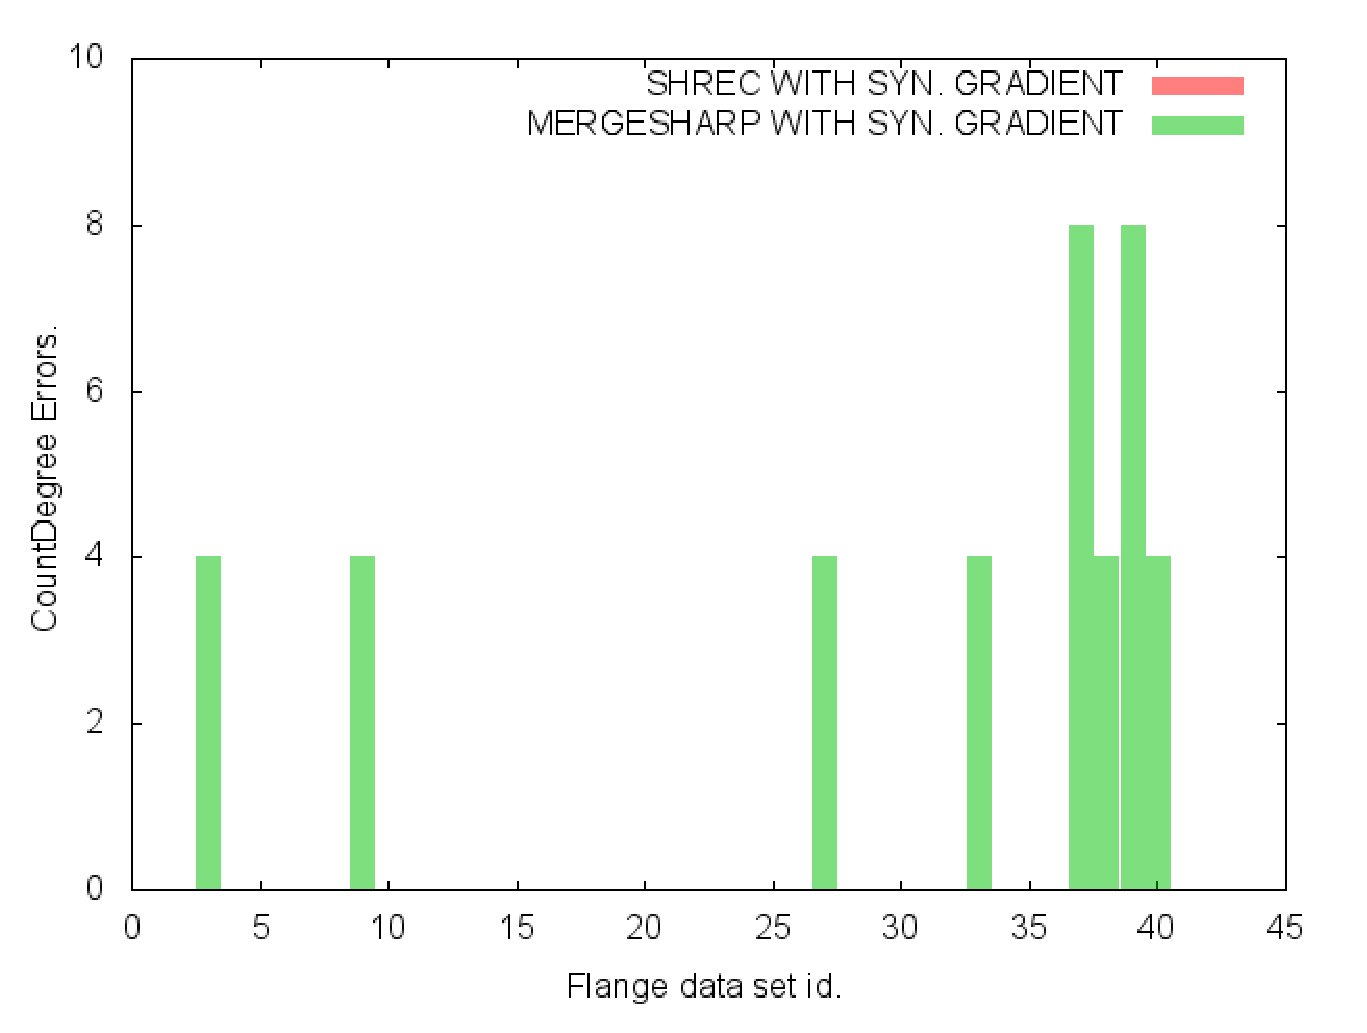
\includegraphics[width=0.8\linewidth]{images/mergeSharpvsShrec.eps}\label{fig:mergesharp:a}}\\
	\subfloat[]{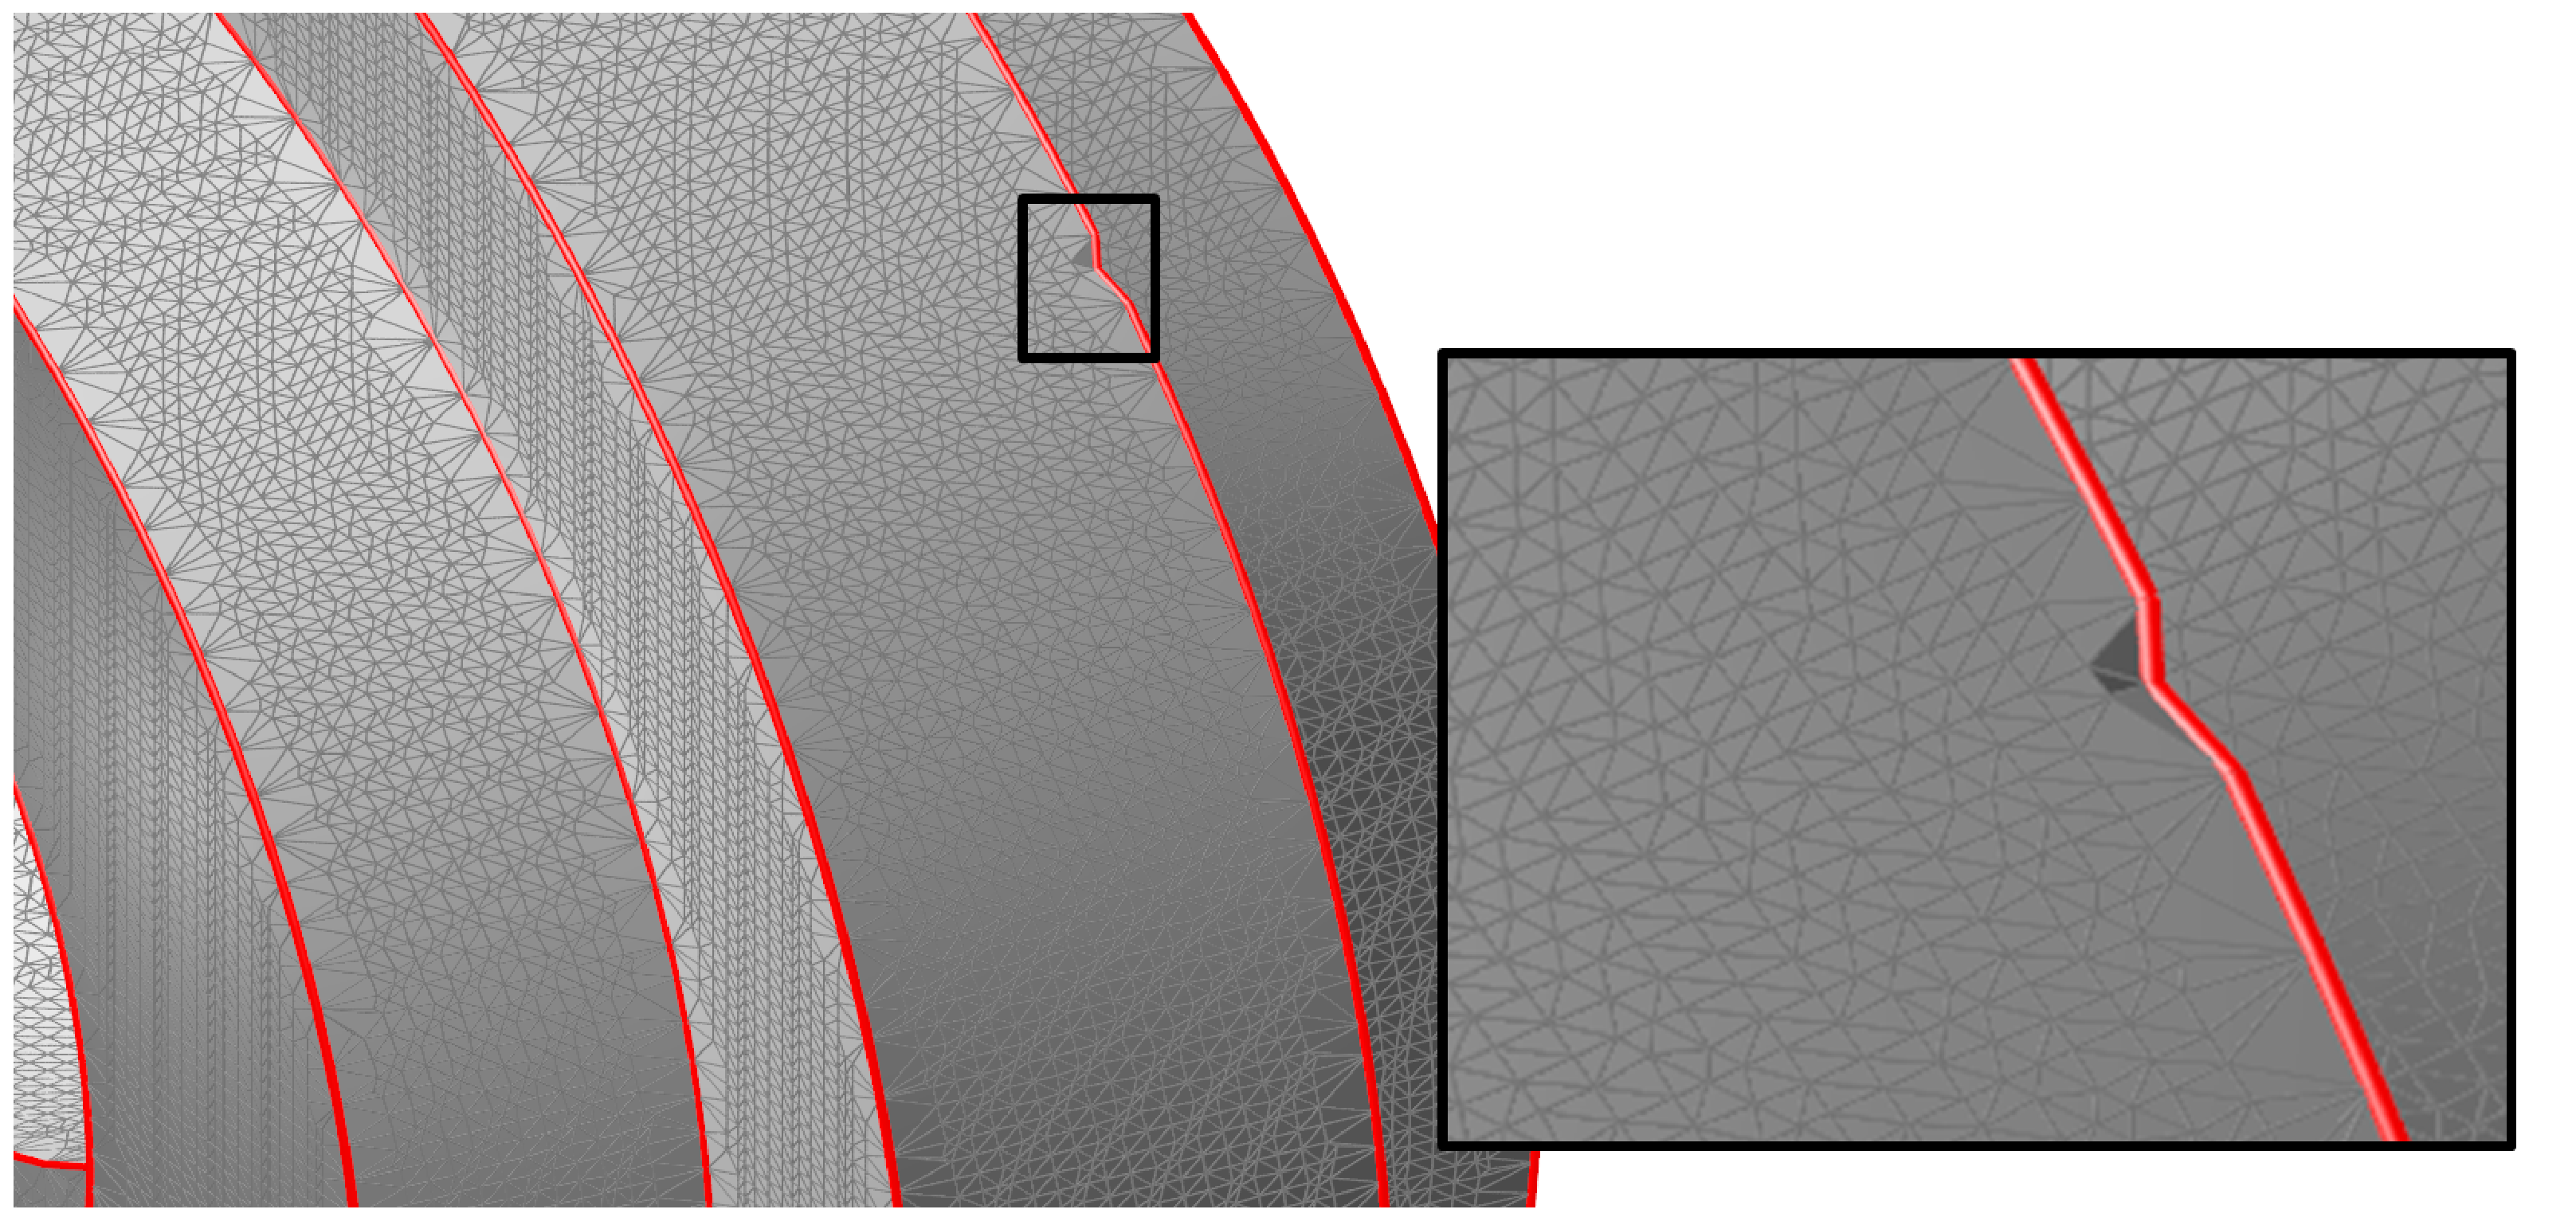
\includegraphics[width=0.6\linewidth]{images/mergeSharpvsShrec2.eps}\label{fig:mergesharp:b}}\\
	\subfloat[]{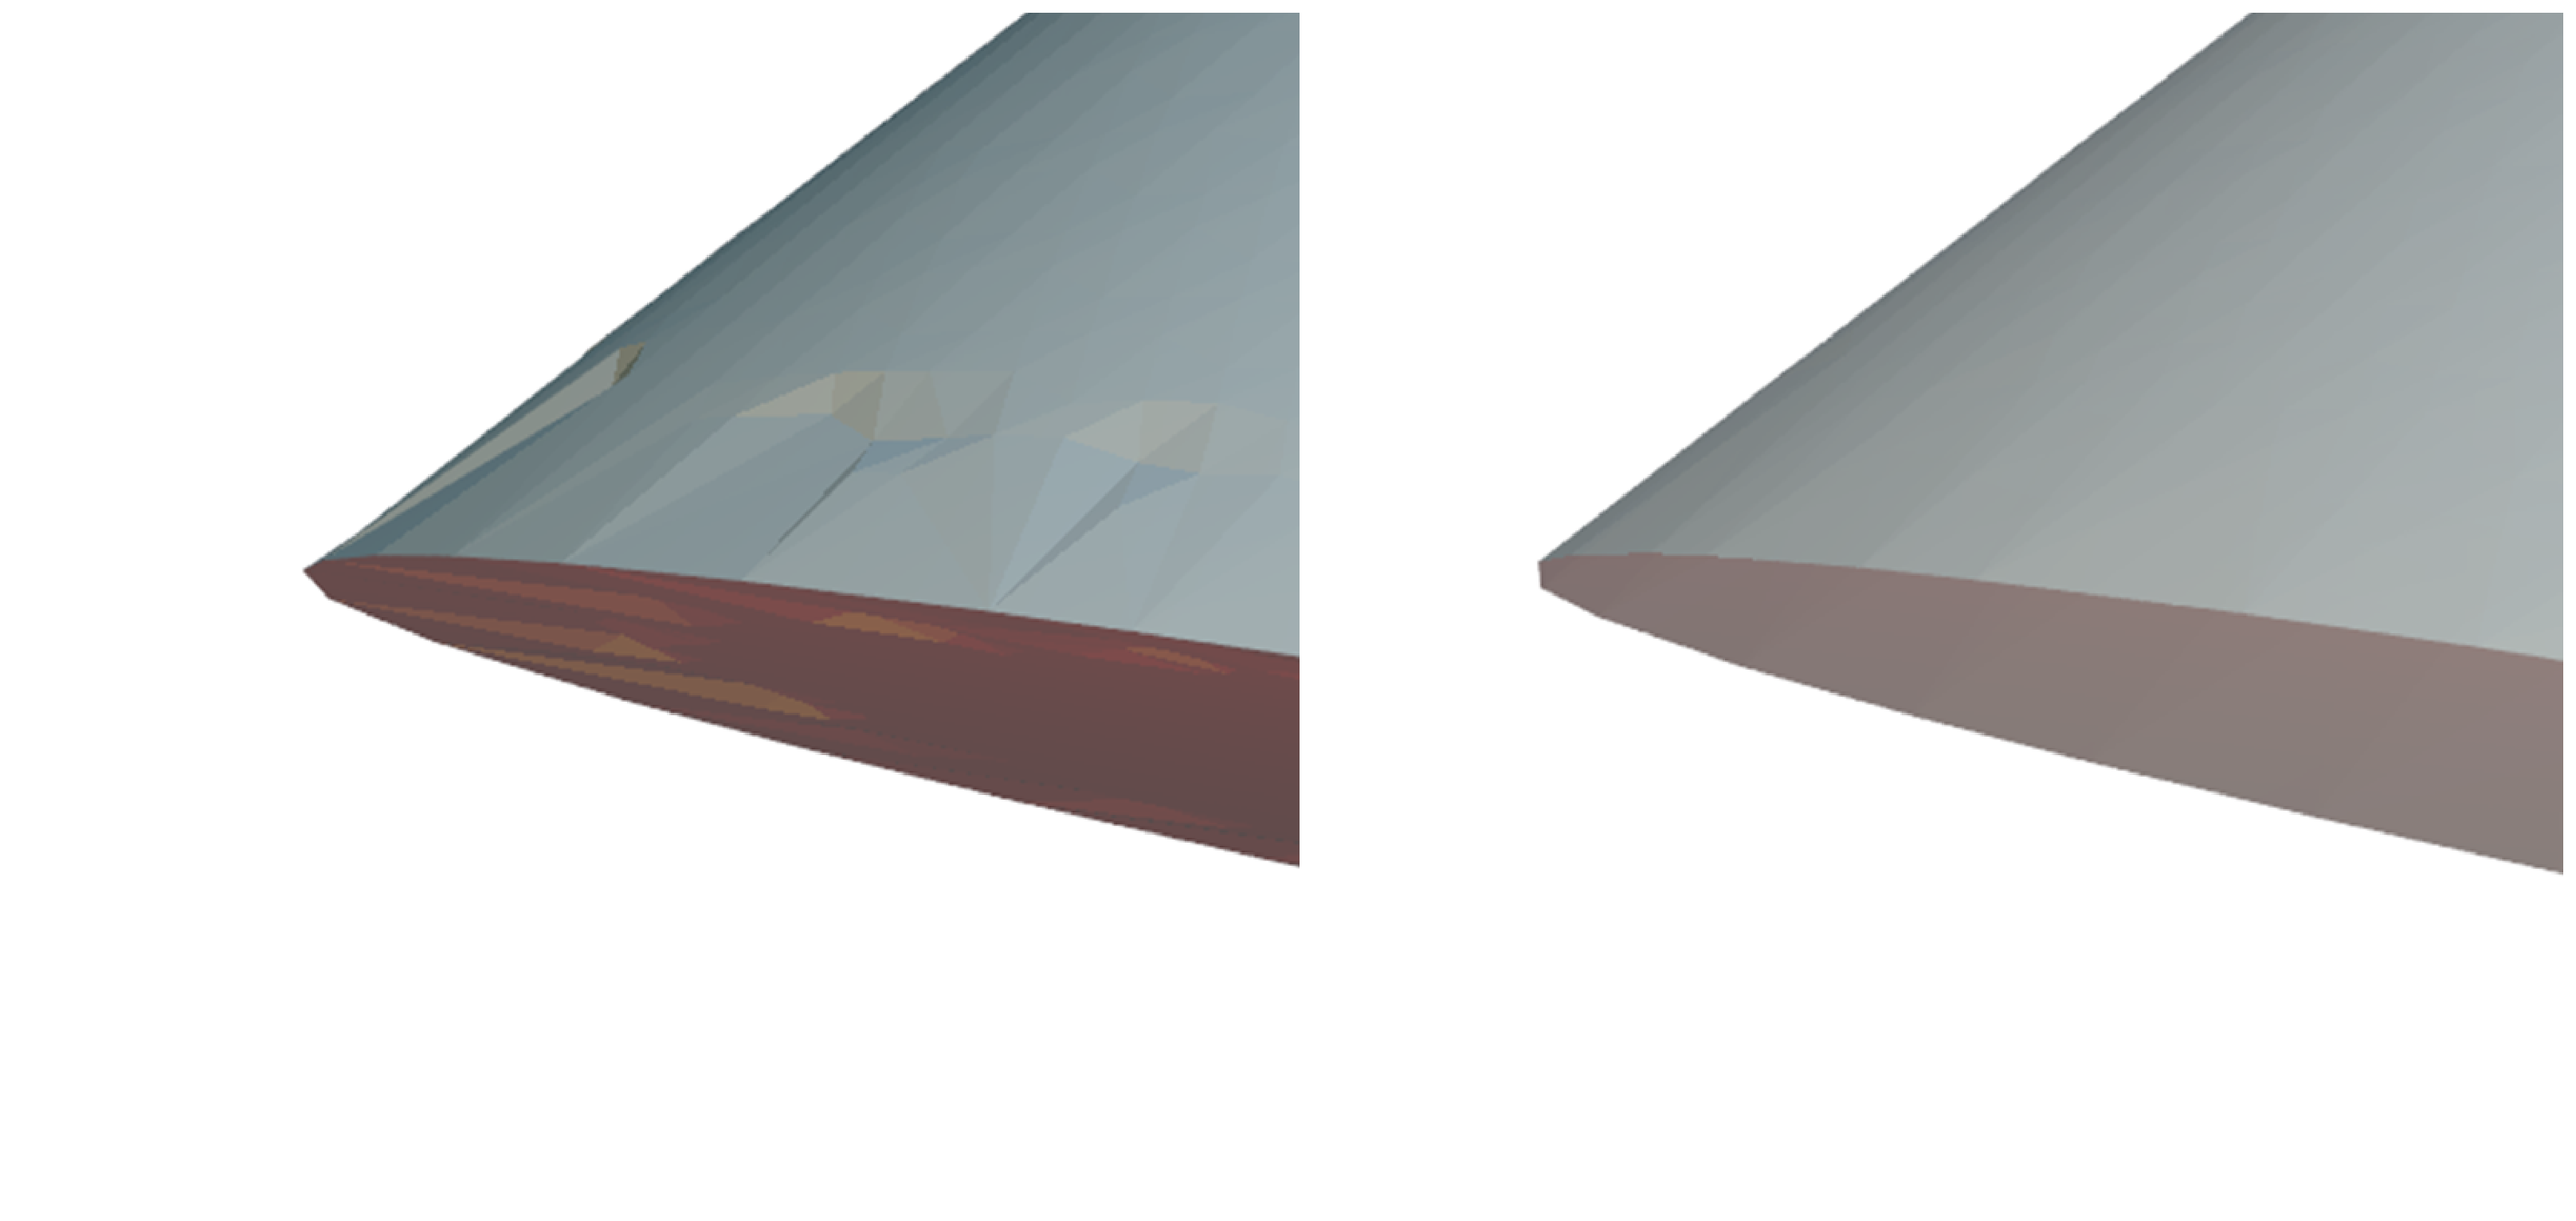
\includegraphics[width=0.6\linewidth]{images/cone_mergesharp.eps}\label{fig:mergesharp:c}}
	\caption{Result of  MERGESHARP and SHREC with synthetic gradients. (a) Summary results of  CountDegree errors of 40 Flange datasets. SHREC does not produce an errors. (b) Result on one particular data set using MERGESHARP, magnified region shows one of the ``notches" created. (c) Apart from ``Notches", MERGESHARP produces gentle dimples which decays the visual quality. Magnified region shows a portion of a Cone dataset (Left) MERGESHARP (Right) SHREC. }
	\label{fig:mergeSharpVShrec}
\end{figure}	
We first compare our algorithm with MERGESHARP ~\cite{bw-cisec-13}, Figure~\ref{fig:mergeSharpVShrec} shows the result. Figure~\protect\subref*{fig:mergesharp:a} shows the summary of CountDegree results of running MERGESHARP on 40 Flange datasets. SHREC as discussed above does not generate any errors. Figure~\protect\subref*{fig:mergesharp:b} shows the result on one of the Flange data sets. MERGESHARP produces ``notches" such as the one shown. 

MERGESHARP also produces gentle dimples such as the ones in the edge of a Cone data set shown in Figure~\protect\subref*{fig:mergesharp:c}, SHREC does not produce them. 	
\paragraph{Comparison with Cocone}
We compare our algorithm to the algorithm WeightCocone by Dey et al.~\cite{Dey2012}. WeightCocone reconstructs a surface with sharp edges and corners from a sampled point cloud. WeightCocone takes two inputs; one contains the point cloud, another is a weighted sampling of feature curves. Weight of the sampling will be used as weight of the protecting balls. WeightCocone generates as output a feature sensitive mesh. 

The feature curve (second input to WeightCocone) is constructed using the algorithm FeatureRecon by Dey et al.~\cite{Dey2013}. FeatureRecon extracts feature curves of a surface. The input is a point cloud sampled on the surface. FeatureRecon has two steps, feature point detection and feature curves reconstruction. 
\paragraph{Experimental details:} The input to FeatureRecon is a point cloud. We tested two different input point cloud;
\begin{enumerate}
	\item We applied Marching Cubes~\cite{lc-mchr3-87} on our datasets Sec.\ref{sec:synData}. The vertices of the mesh generated by the Marching Cubes algorithm are then super-sampled using the Monte Carlo point sampling, to generate a point cloud with approximately sixty-five thousand points.
	\item We super-sampled the ``perfect" meshes Sec.\ref{sec:synData}, to generate generate a point cloud with approximately sixty-five thousand points.
\end{enumerate}
The two different point clouds are used as input to FeatureRecon to extract the feature curves. 
FeatureRecon has nine separate parameters. Experimentally and also noted by the authors Dey et al.~\cite{Dey2013}, we found FeatureRecon to be heavily reliant on parameter fine tuning. We used the following parameter values for our TwoCube datasets, (as suggest by the authors Dey et al.~\cite{Dey2013}). 
$-t = 25,-fl = 0.04, -cl = 0.06, -dc = 0, -\rho3 = 0.32, -\rho1 = 0.0, -rc = 3$.

The feature curves generated using FeatureRecon along with the super-sampled point cloud is used as input to WeighCocone. For comparison test, we compare the known ``perfect" mesh with the output of WeightCocone. 
We report the degree count of the ``sharp" edges (dihedral angle less than $140^\circ$). We also report the surface angle distances between the output and the perfect mesh. 
\begin{figure}[t] 
	%dataset t110 reconstructed from perfect mesh 
	\centering  	
	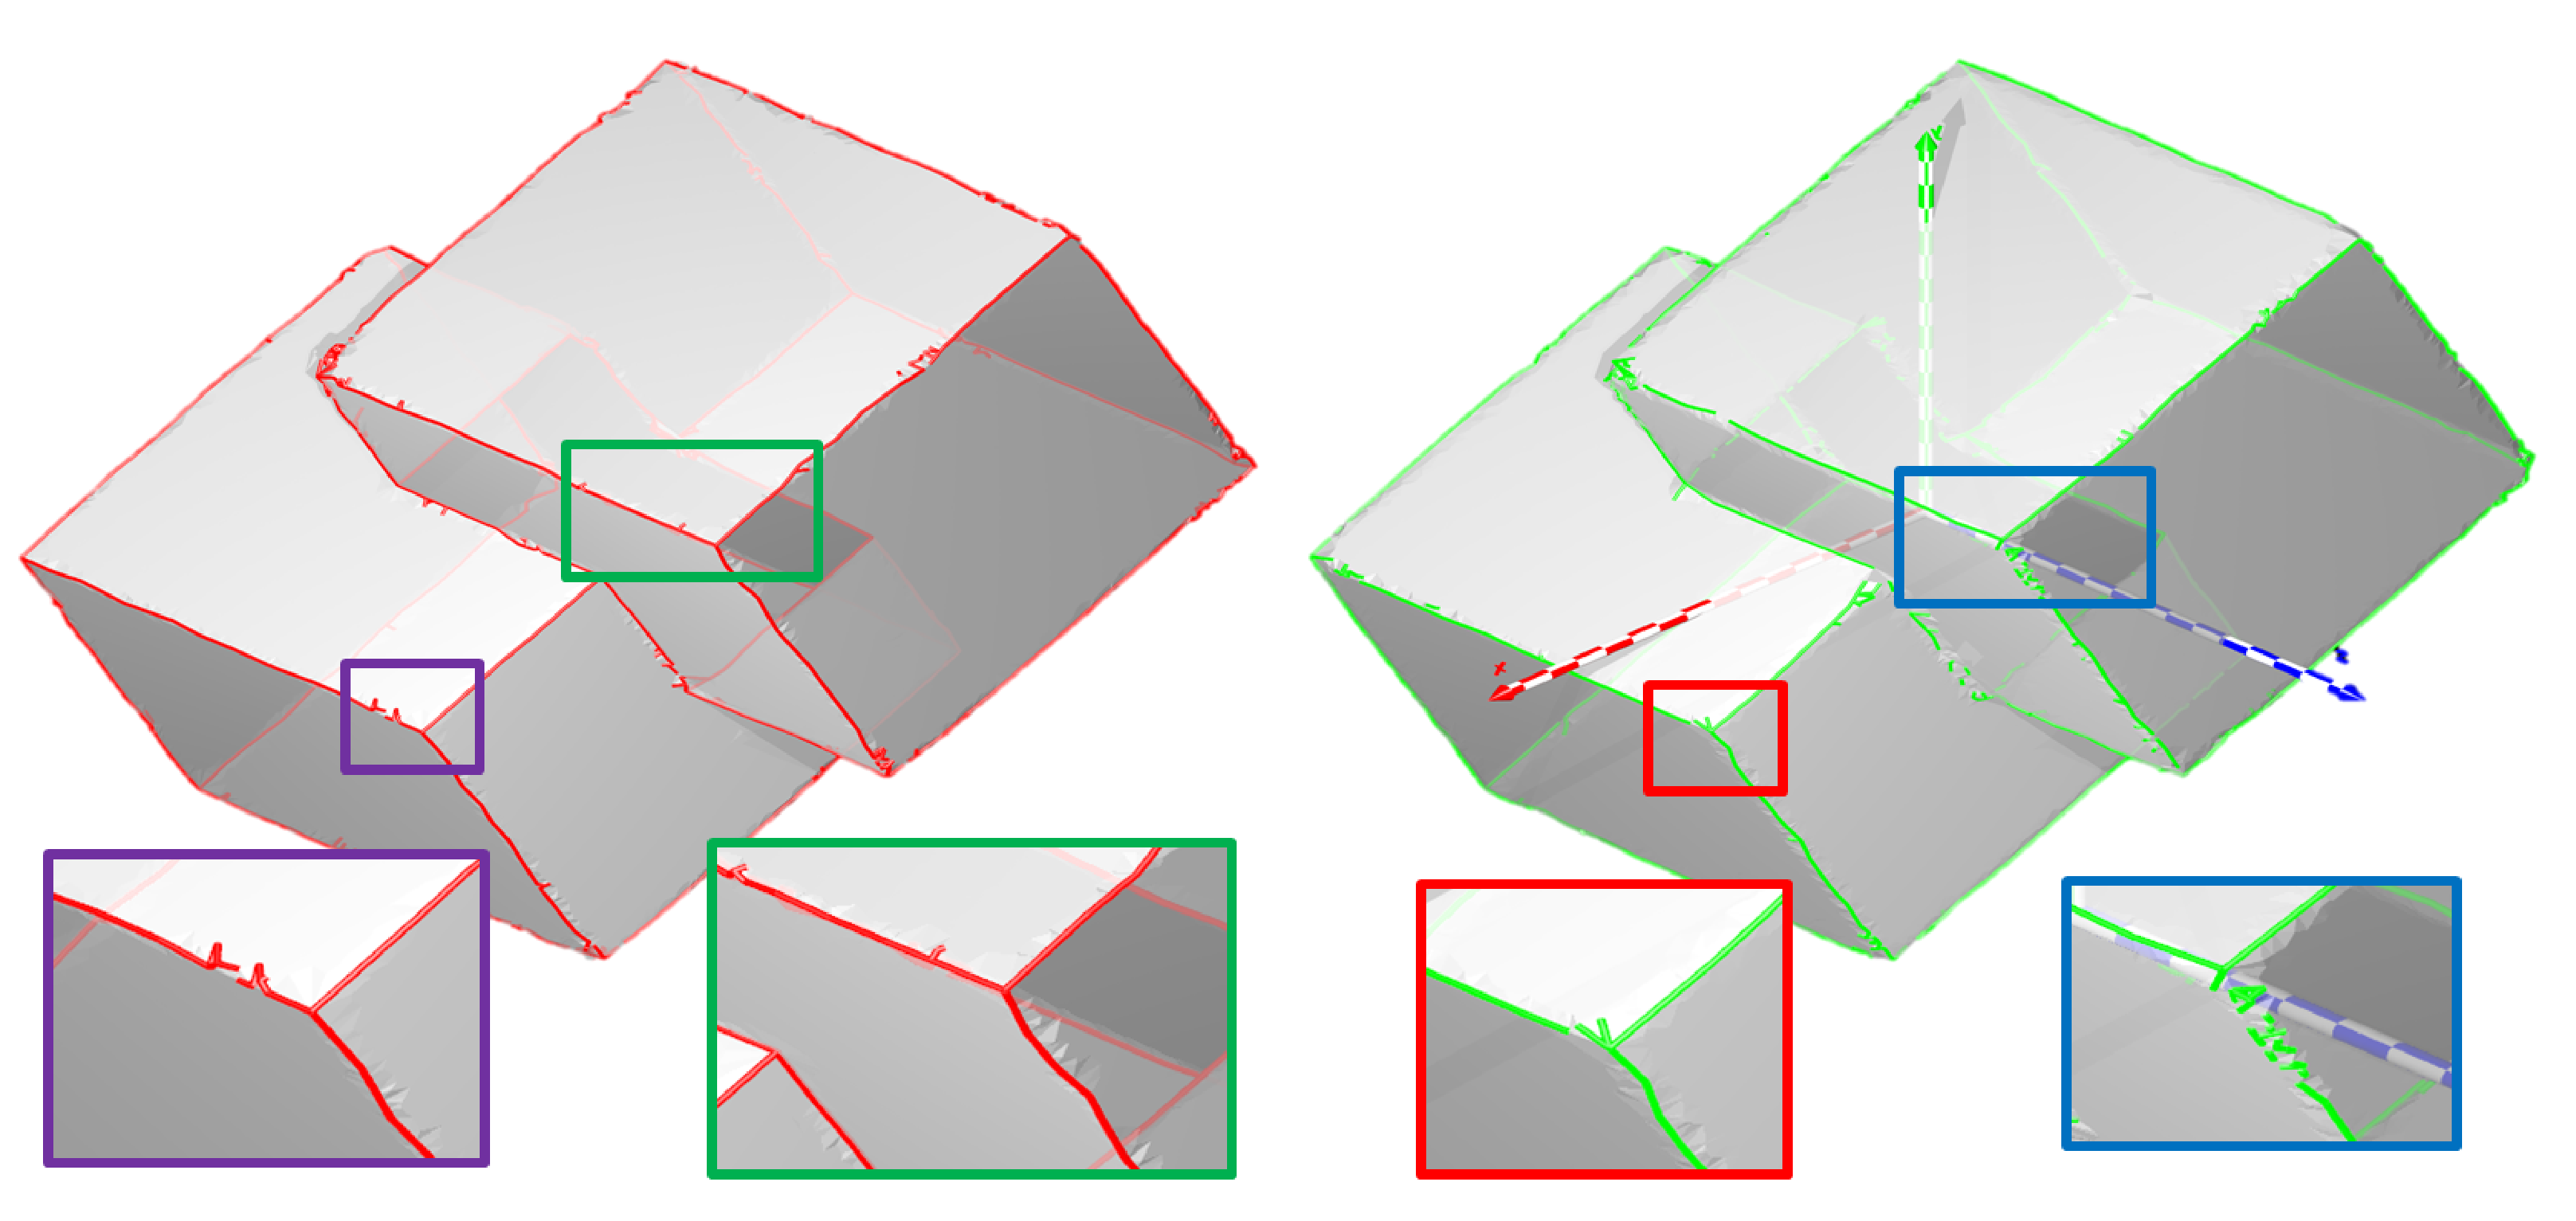
\includegraphics[width=\linewidth]{images/compare_cocone_perfect_mc.eps}
	\caption{Result of WeightCocone reconstruction on a TwoCube dataset (id 110). (a) Input cloud is the super-sampled ``perfect" mesh. (b) Input cloud is the super-sampled Marching Cube mesh. The magnified regions show some of the errors. The reconstruction from point cloud generated from the Marching Cube input is worse than the  point cloud from ``perfect" mesh input. }
	\label{fig:cocone_compare_from_perfect_1}
	\vskip-0.2cm
\end{figure} 
Figure~\ref{fig:cocone_compare_from_perfect_1} shows the reconstructed mesh for dataset id 110. The associated ``sharp" edges are also shown. Figure~\ref{fig:cocone_compare_from_perfect_1}(a) shows the reconstruction from the point cloud generated from the ``perfect" mesh. The overlay-ed ``sharp" edges (in red) show that the reconstruction has many errors. The magnified regions show some of the errors along the sharp edges and corners. Figure~\ref{fig:cocone_compare_from_perfect_1}(b) shows the reconstruction from the point cloud generated from running Marching Cubes. The magnified regions show the same regions as Figure~\ref{fig:cocone_compare_from_perfect_1}(a). The reconstruction is worse than WeightCocone using input from perfect mesh. 

Figure~\protect\subref*{table:cocone_compare_with_mc_table_2} shows the angular difference from the ``perfect" mesh to those generated by WeightCocone using points sampled from the ``perfect" mesh,  over a randomly selected subset of 21 cases out of the 143 TwoCube datasets. The number of simplices with more than 30$^\circ$, 40$^\circ$ and 50$^\circ$ errors from the original mesh are shown. Figure~\protect\subref*{fig:shrecTwoCube:a},~\protect\subref*{fig:shrecTwoCube:c} show that algorithm SHREC generates far fewer errors and with smaller angle difference to the original mesh. WeightCocone when using Marching Cubes point cloud as input produces worse results and is not shown.

Figure~\protect\subref*{table:cocone_compare_with_mc_table_1} shows the results on a single dataset, the same as in Figure~\ref{fig:cocone_compare_from_perfect_1}. The surface angle difference from the original mesh while using the three algorithms; WeightCocone with inputs points super-sampled from the original mesh, WeightCocone with points input points super-sampled from the Marching cubes mesh and SHREC. 
WeightCocone using points sampled from the perfect mesh produces a considerable number of errors. WeightCocone using the points sampled from the Marching cubes is even worse. 
SHREC on same dataset produces no errors ( see Figure~\ref{fig:shrecPerfect1}). 

Dey et al.~\cite{Dey2012,Dey2013} report better results on their datasets, Which might possibly be because of parameter tuning. They themselves acknowledged as such in their work.
\begin{figure}[tb]
	\centering
		\subfloat[]{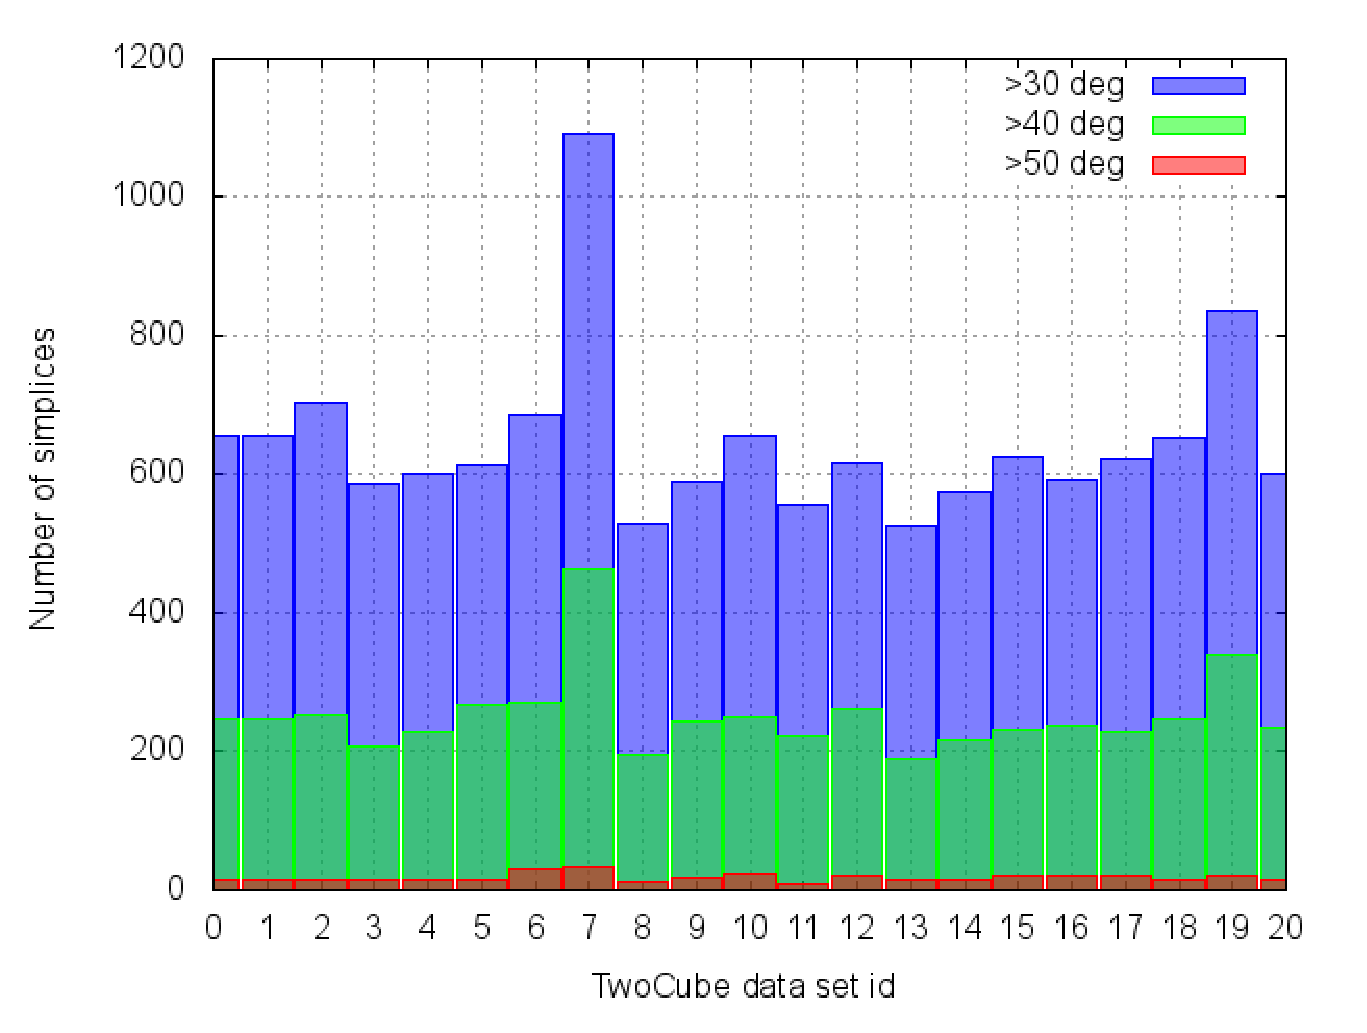
\includegraphics[width=0.6\linewidth]{images/num_simplices_large_test_twoCube.eps}\label{table:cocone_compare_with_mc_table_2}}\\
		\subfloat[]{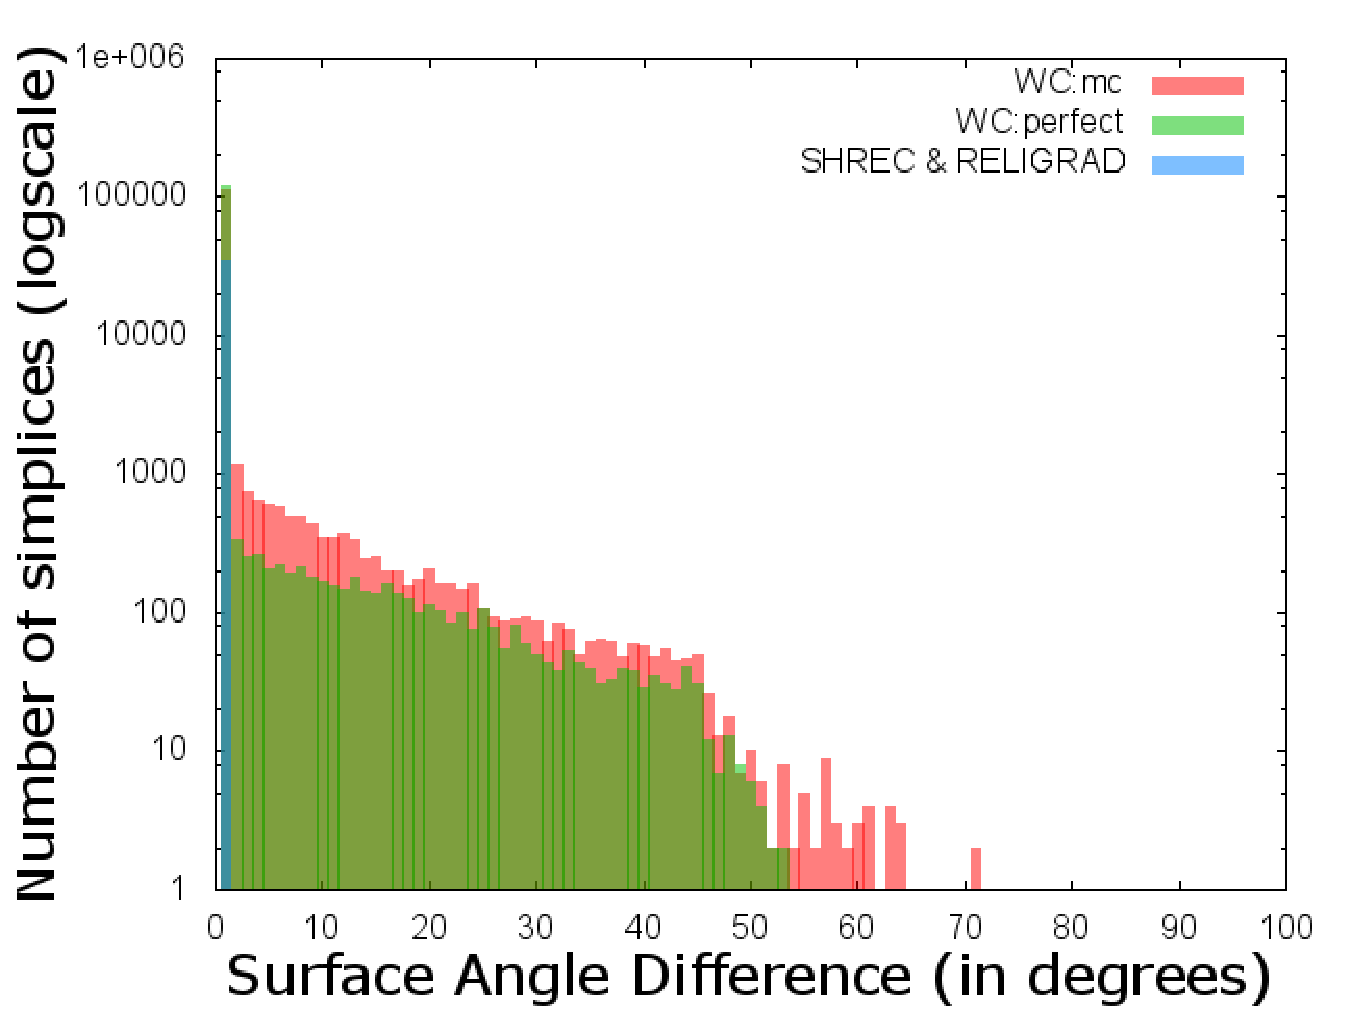
\includegraphics[width=0.6\linewidth]{images/twoCubeQuant.eps}\label{table:cocone_compare_with_mc_table_1}}
		\caption{Cocone comparison Dey et al.~\cite{Dey2012,Dey2013}. (a) Number of simplices with angle difference of 30$^\circ$, 40$^\circ$ and 50$^\circ$ from the original mesh on a subset of 21 TwoCube datasets using WeightCocone with  input points sampled from the perfect mesh. (b) Number of simplices and the corresponding angle difference to the original mesh for a single TwoCube dataset, using WeightCocone with input points super-sampled from perfect mesh, WeightCocone with input super-sampled from Marching cubes and SHREC.}
\end{figure}
\paragraph{Polymender comparison;}
We next compared SHREC to Polymender. Polymender is an implementation of mesh repairing algorithm from Ju~\cite{j-rrpm-04}. Figure~\protect\subref*{fig:polymender:b} shows the result of running Polymender on a flange dataset. Polymender creates creases, notches overlapping/degenerate triangles. On the same dataset SHREC with correct gradients and gradient computed from scalar data using RELIGRAD generates ``no" errors, Figure~\protect\subref*{fig:polymender:a} shows the corresponding result. 

We quantitatively compare the surface angle difference between the Polymender and SHREC result with the known perfect mesh. 
The results in Figure~\protect\subref*{fig:polymender:c} shows the results. Polymender produces many simplices which have large angle difference from the perfect mesh. 
\begin{figure}[tb]
	\centering
		\subfloat[]{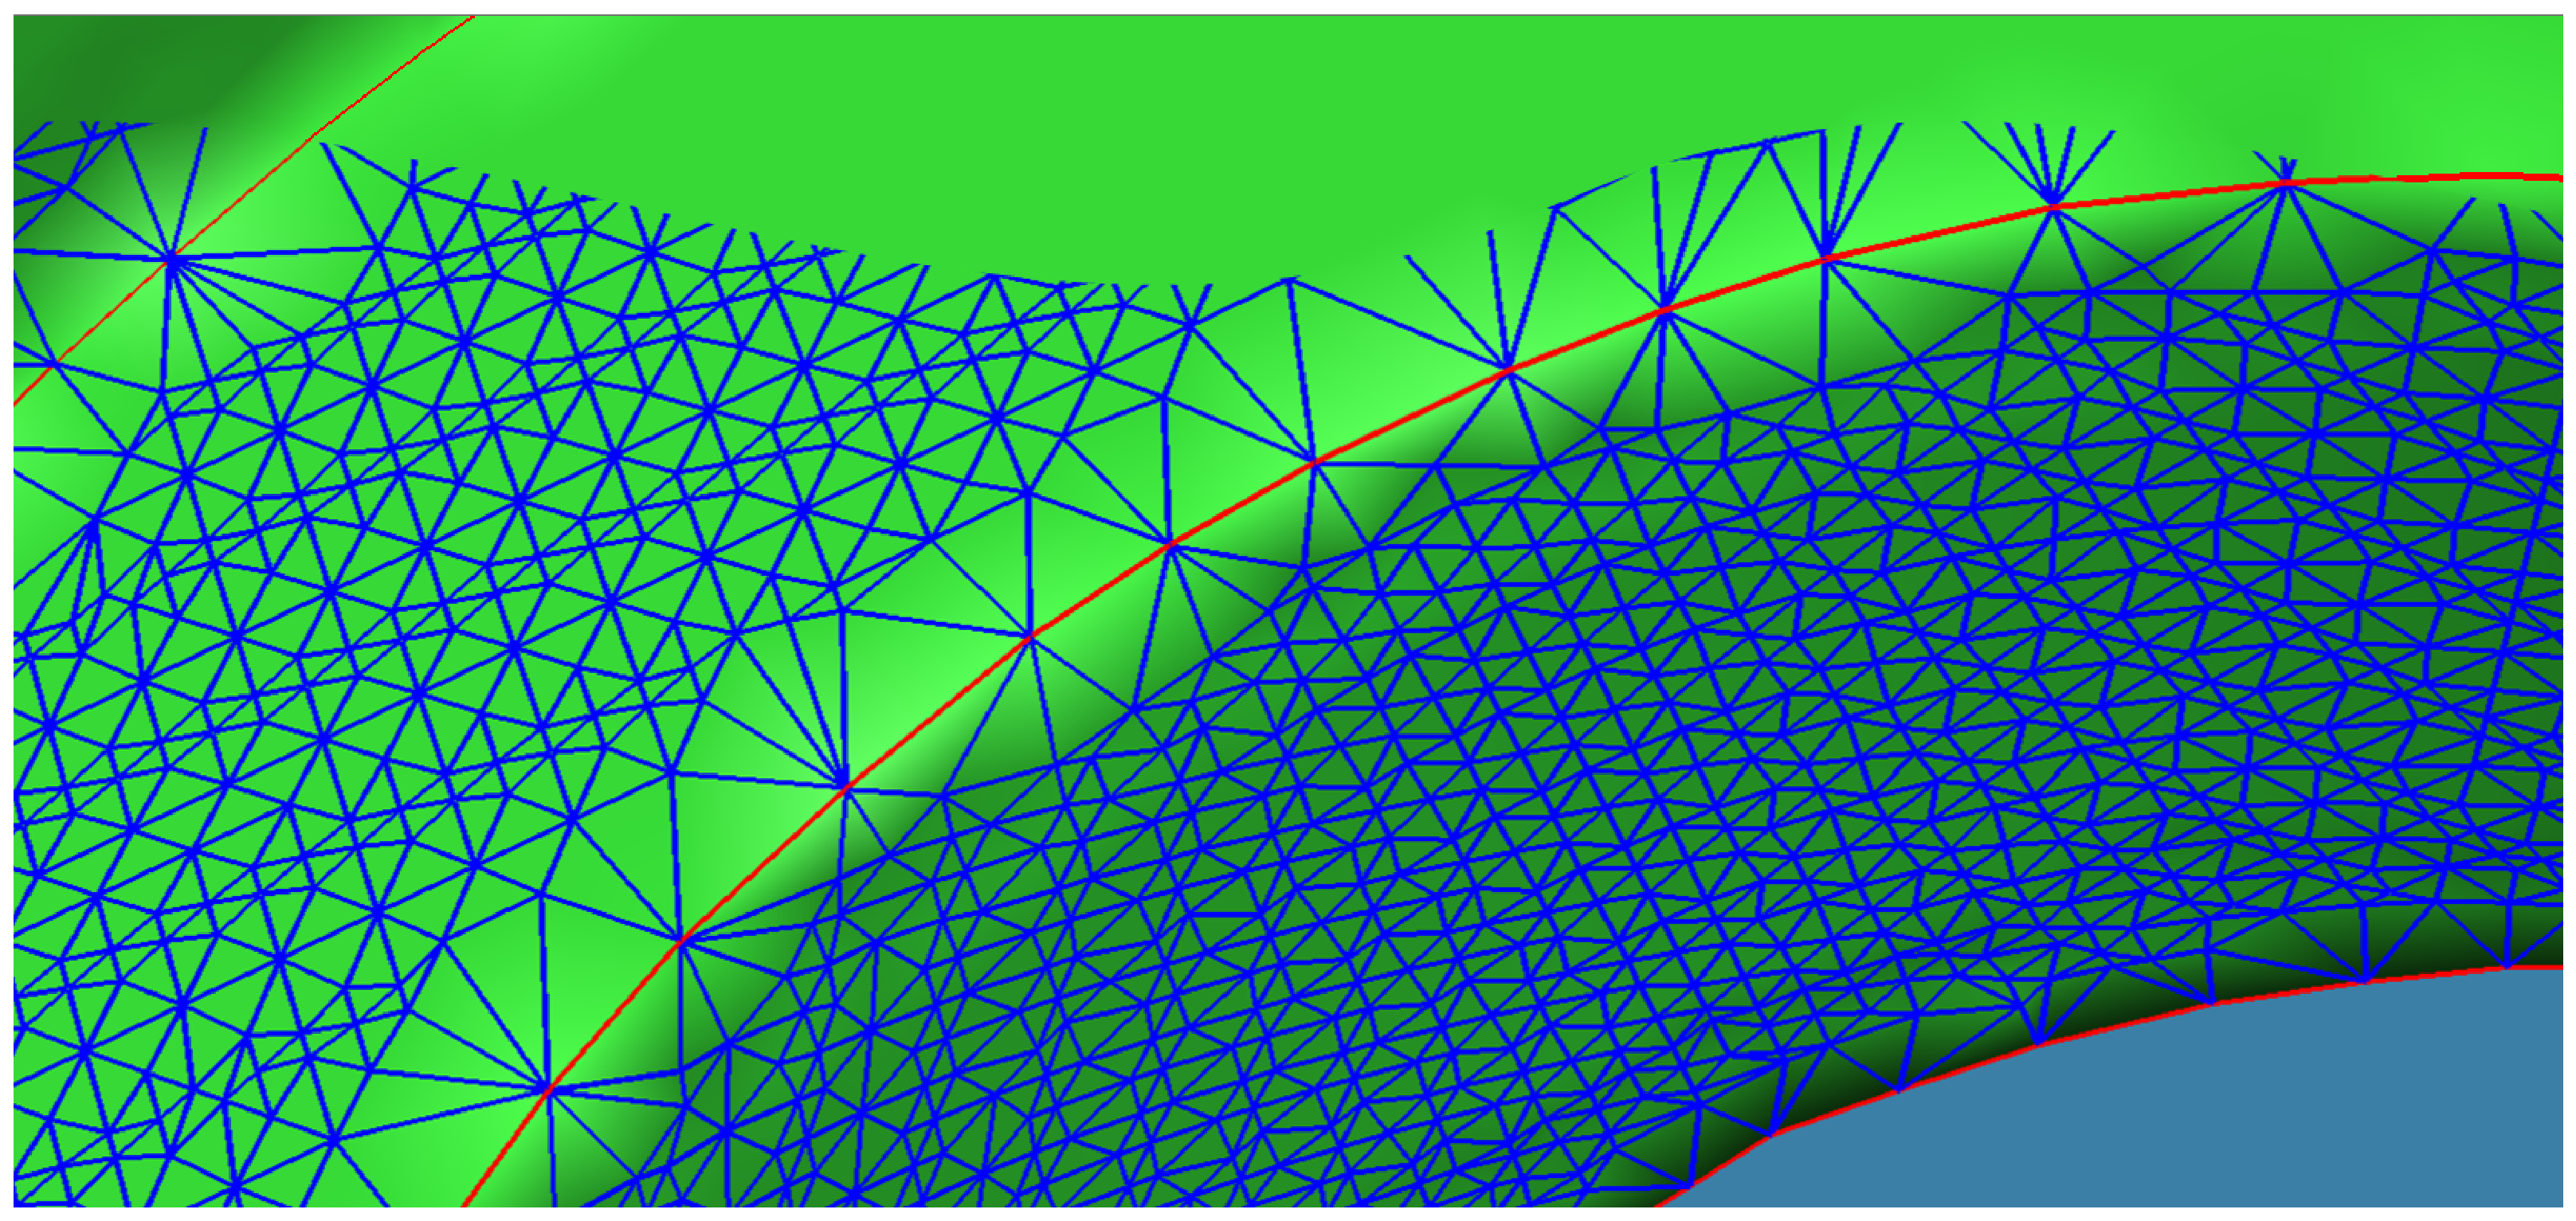
\includegraphics[width=0.45\linewidth]{images/polymender3.eps}\label{fig:polymender:a}}\quad
		\subfloat[]{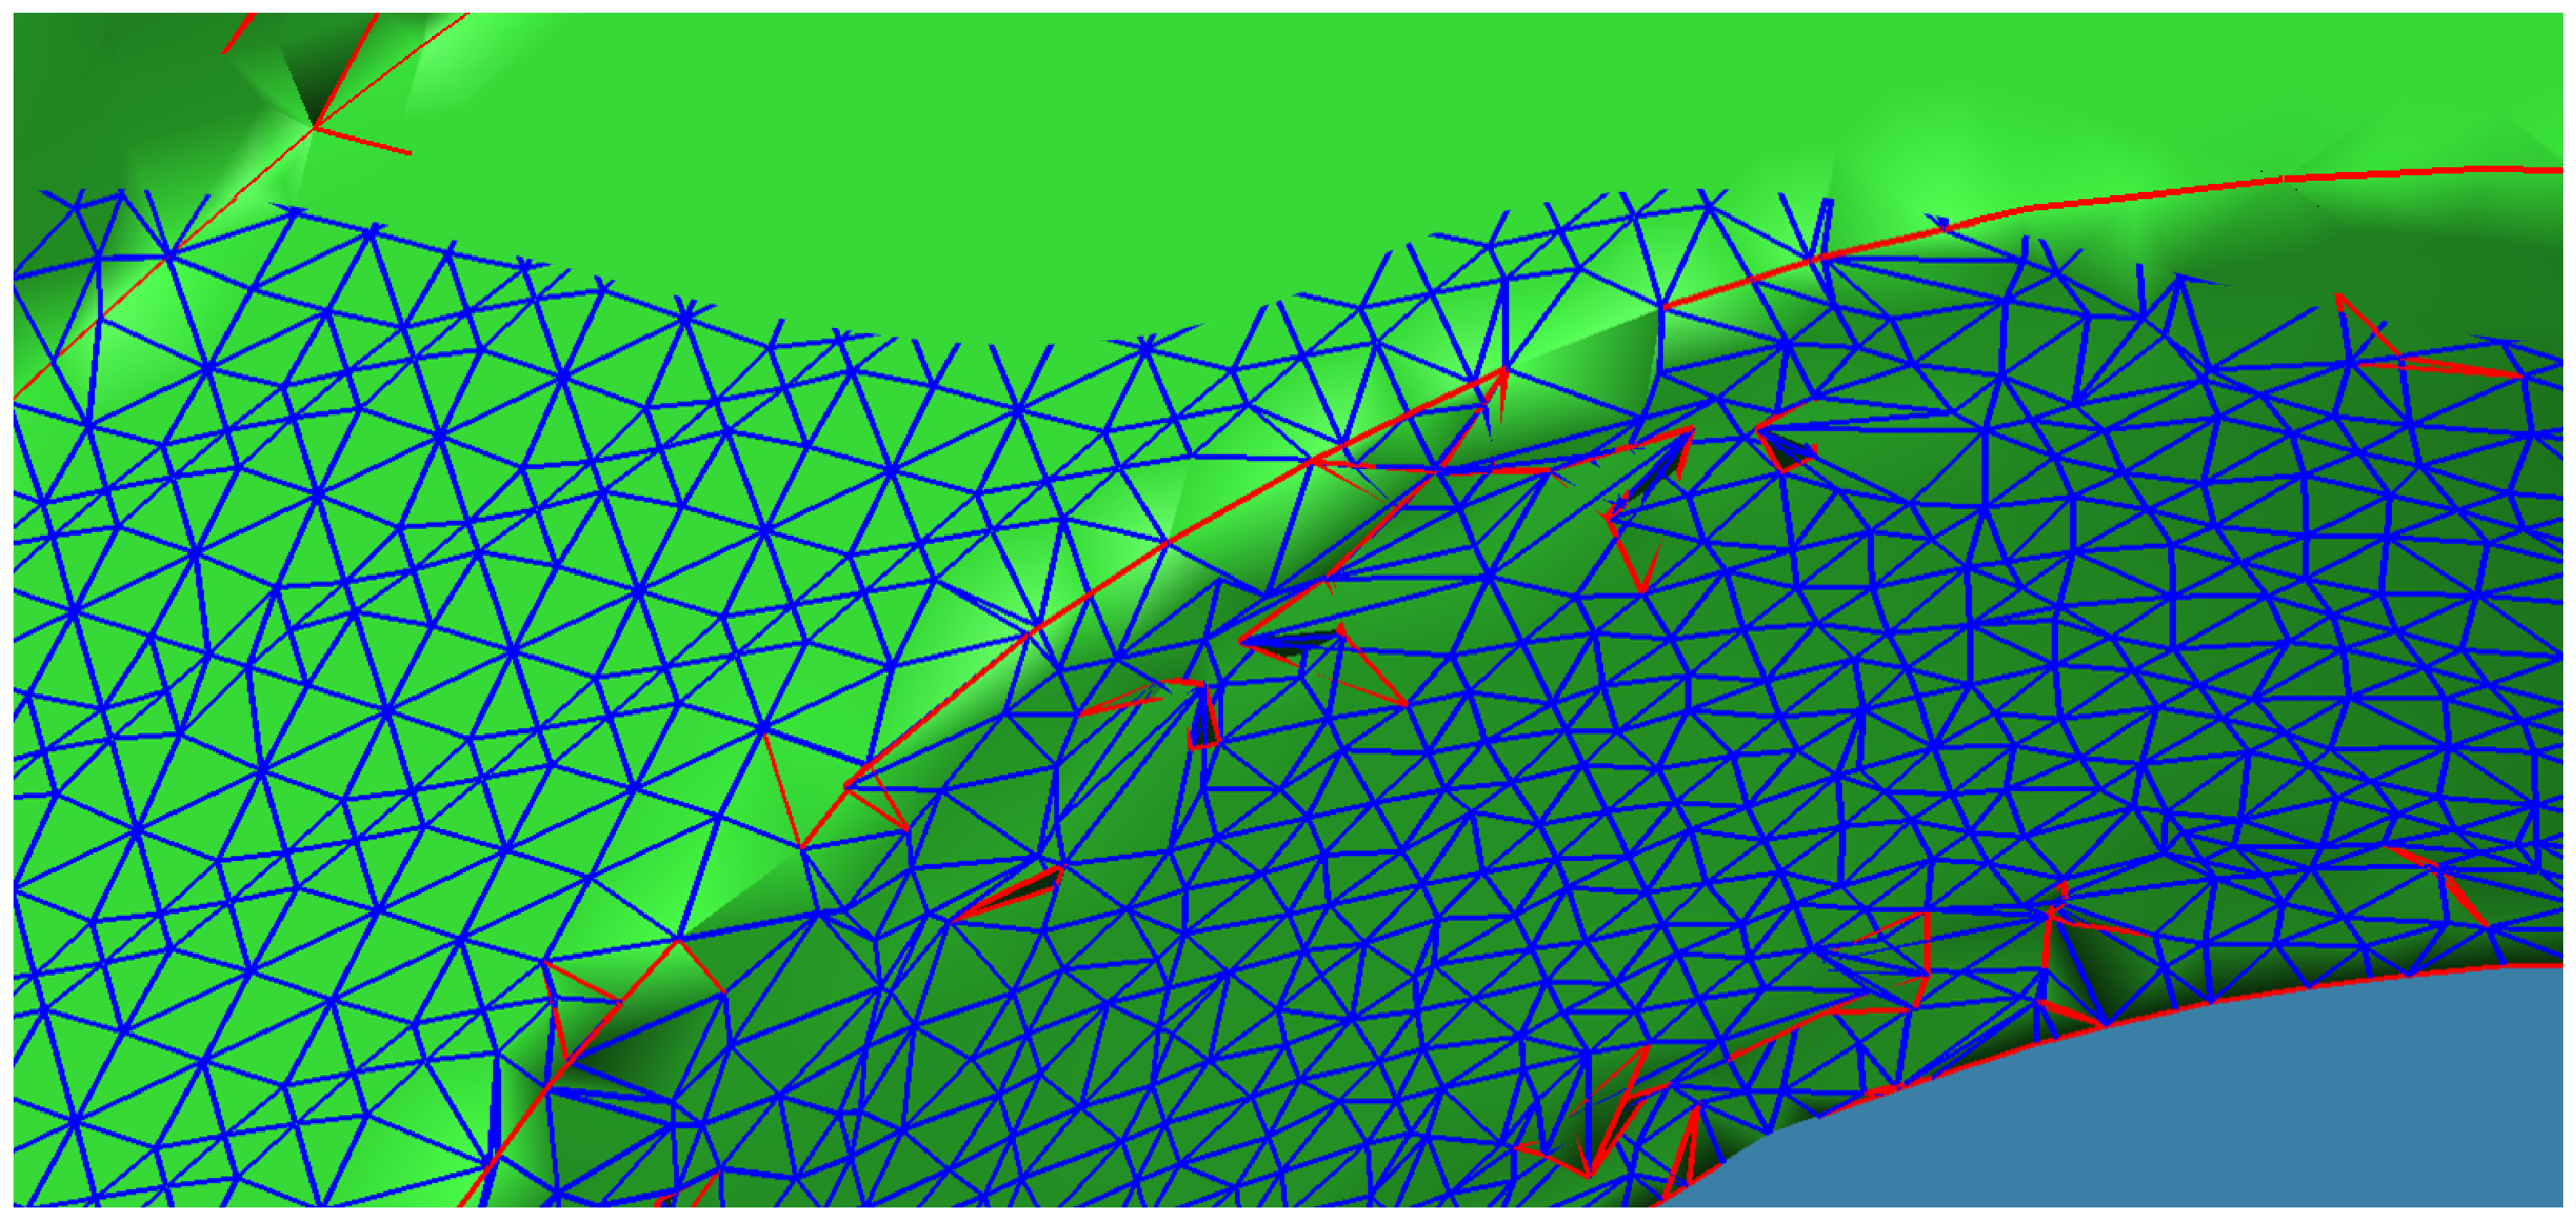
\includegraphics[width=0.45\linewidth]{images/polymender4.eps}\label{fig:polymender:b}}\\
		\subfloat[]{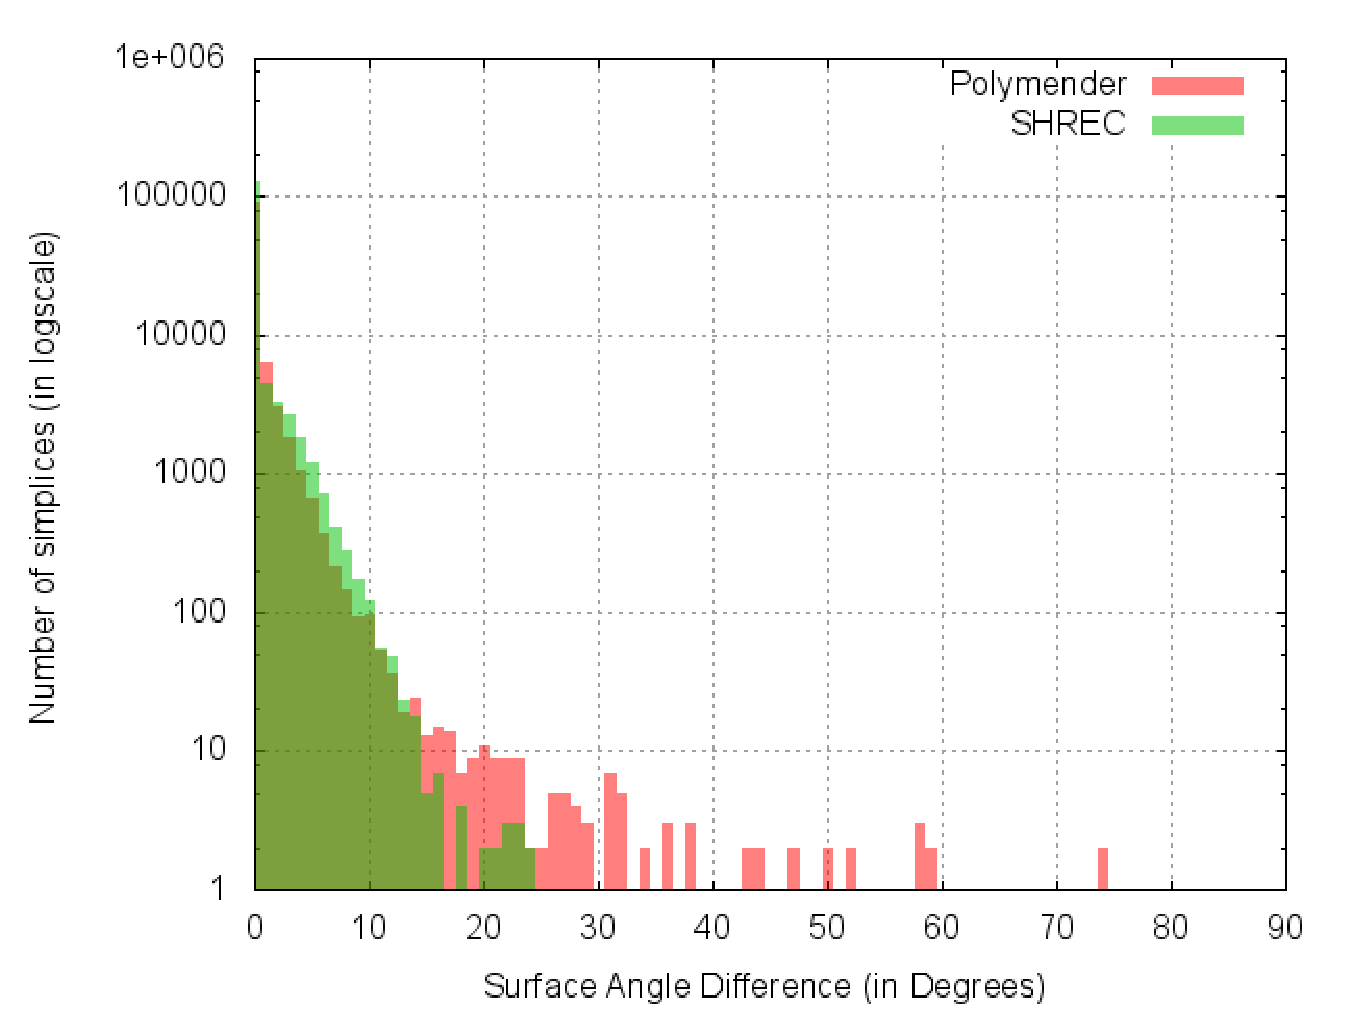
\includegraphics[width=0.7\linewidth]{images/polymenderHistogram_1.eps}\label{fig:polymender:c}}
		\caption{Comparison of Polymender with SHREC on a Flange dataset. The edges with dihedral angle less than $140^\circ$ are overlay-ed in red, a subset of the rest of the edges are overlay-ed in blue. (a) SHREC with RELIGRAD on a part of a flange dataset. (b) Polymender on the same part. (c) Surface angle distance for Polymender and SHREC results from the perfect mesh. Y-axis is in logscale. }	
\end{figure}
\paragraph{Extended Marching Cubes comparison;}
\begin{figure}[tb]
	\centering
	\subfloat[]{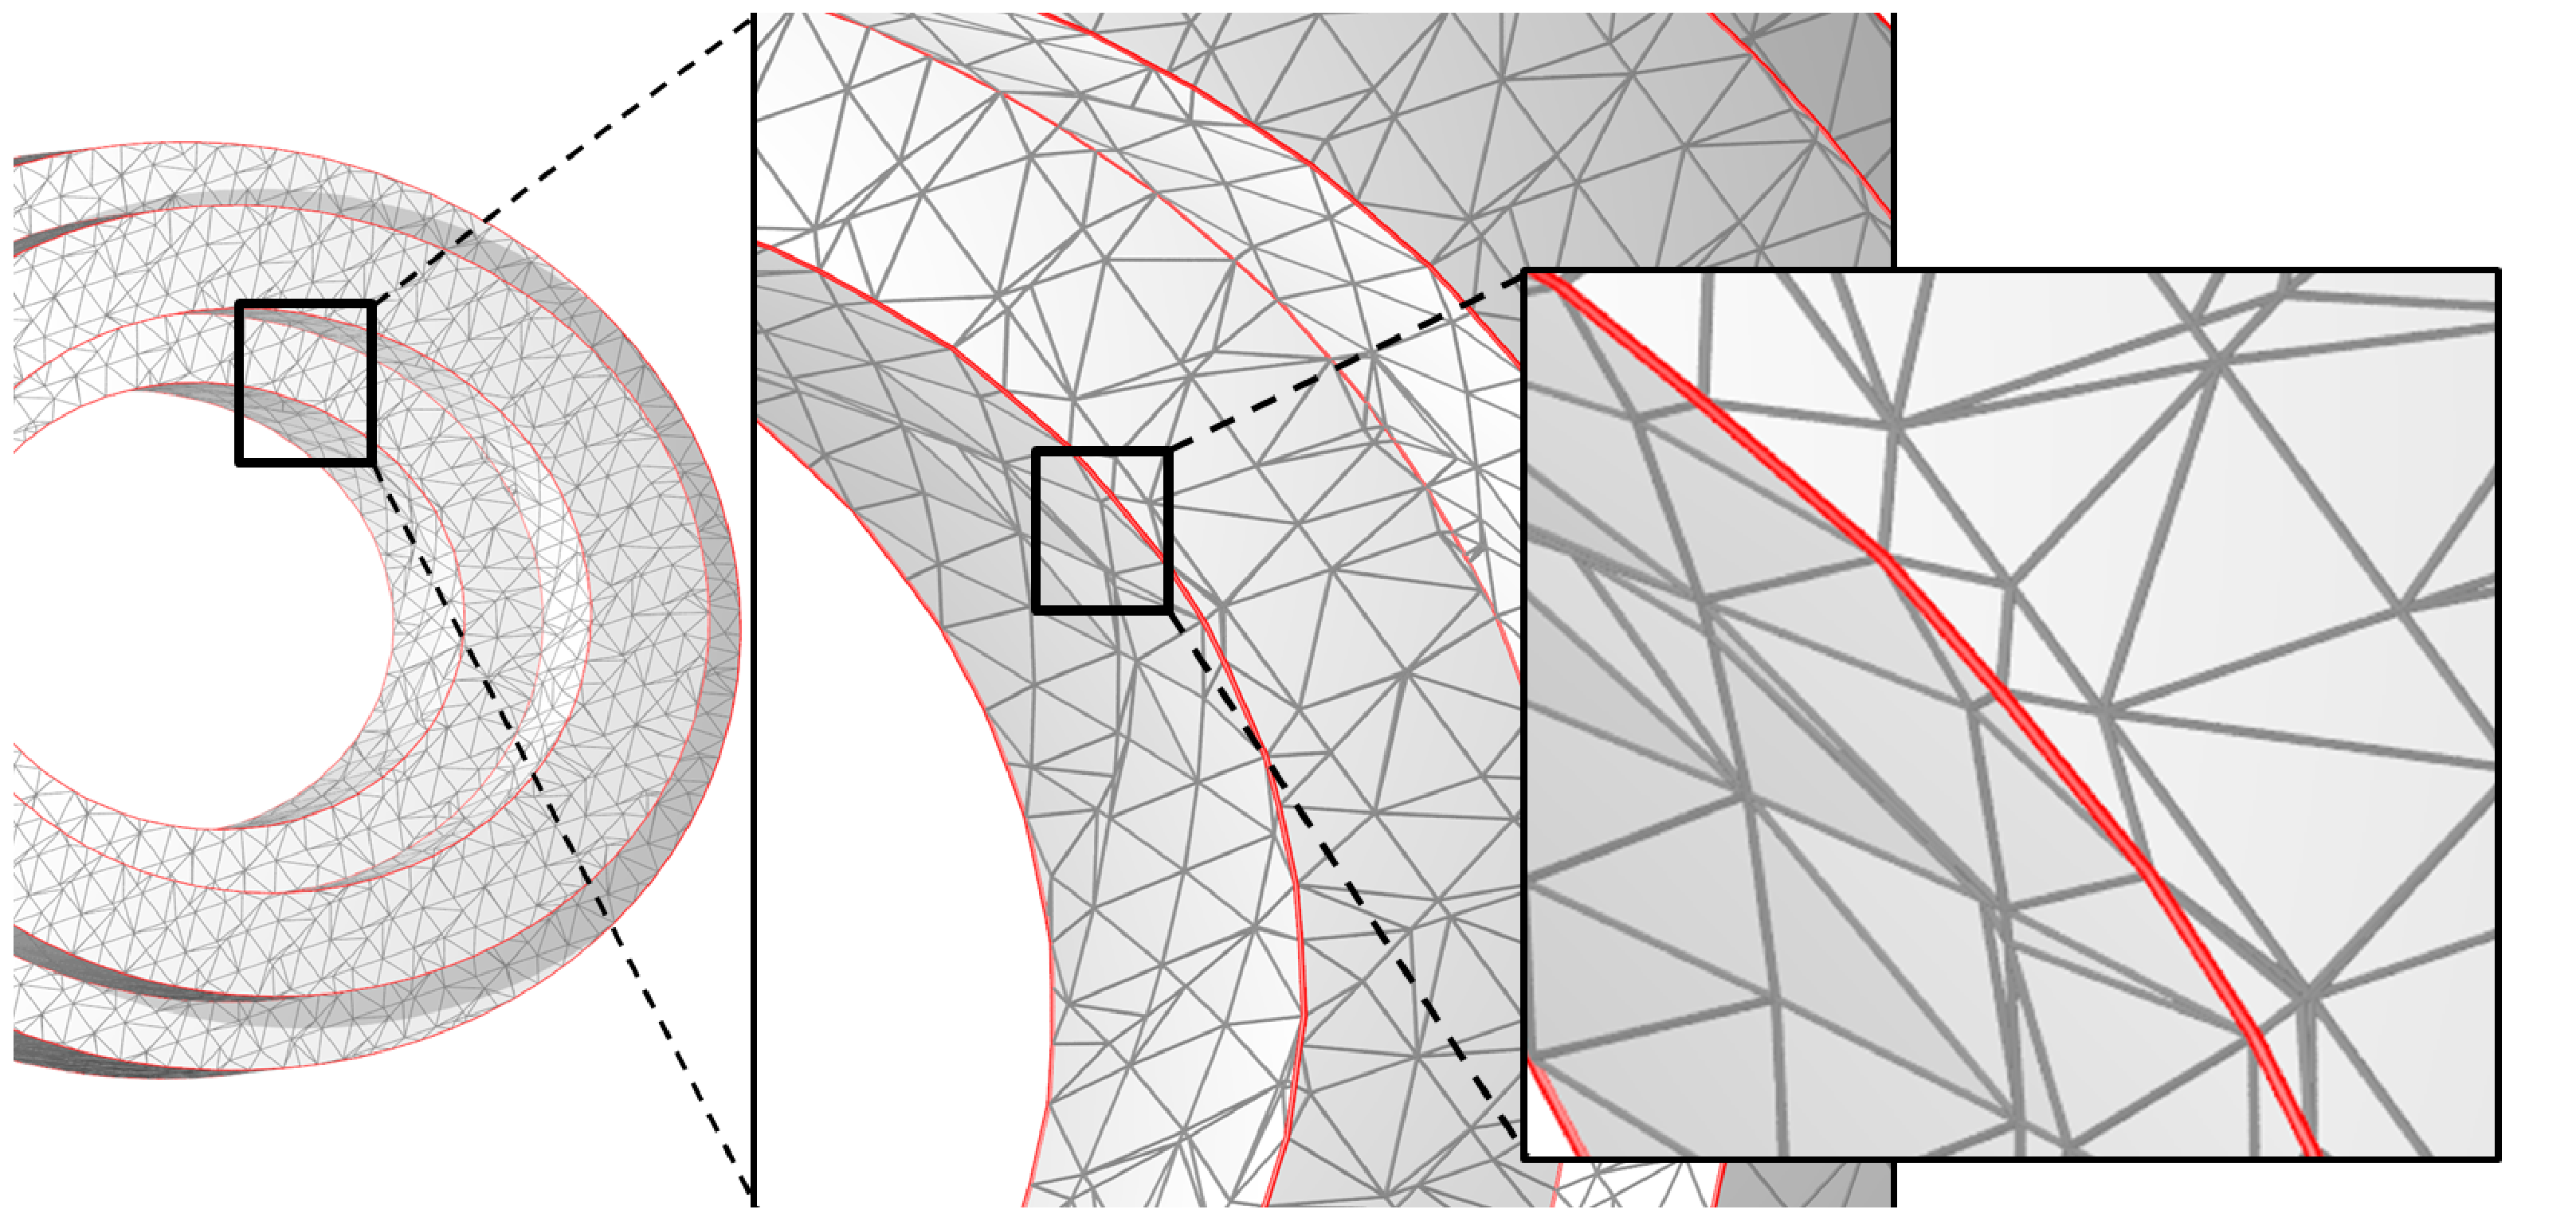
\includegraphics[width=0.7\linewidth]{images/isoExFlange.eps}\label{fig:isoEx:a}}\\
	\subfloat[]{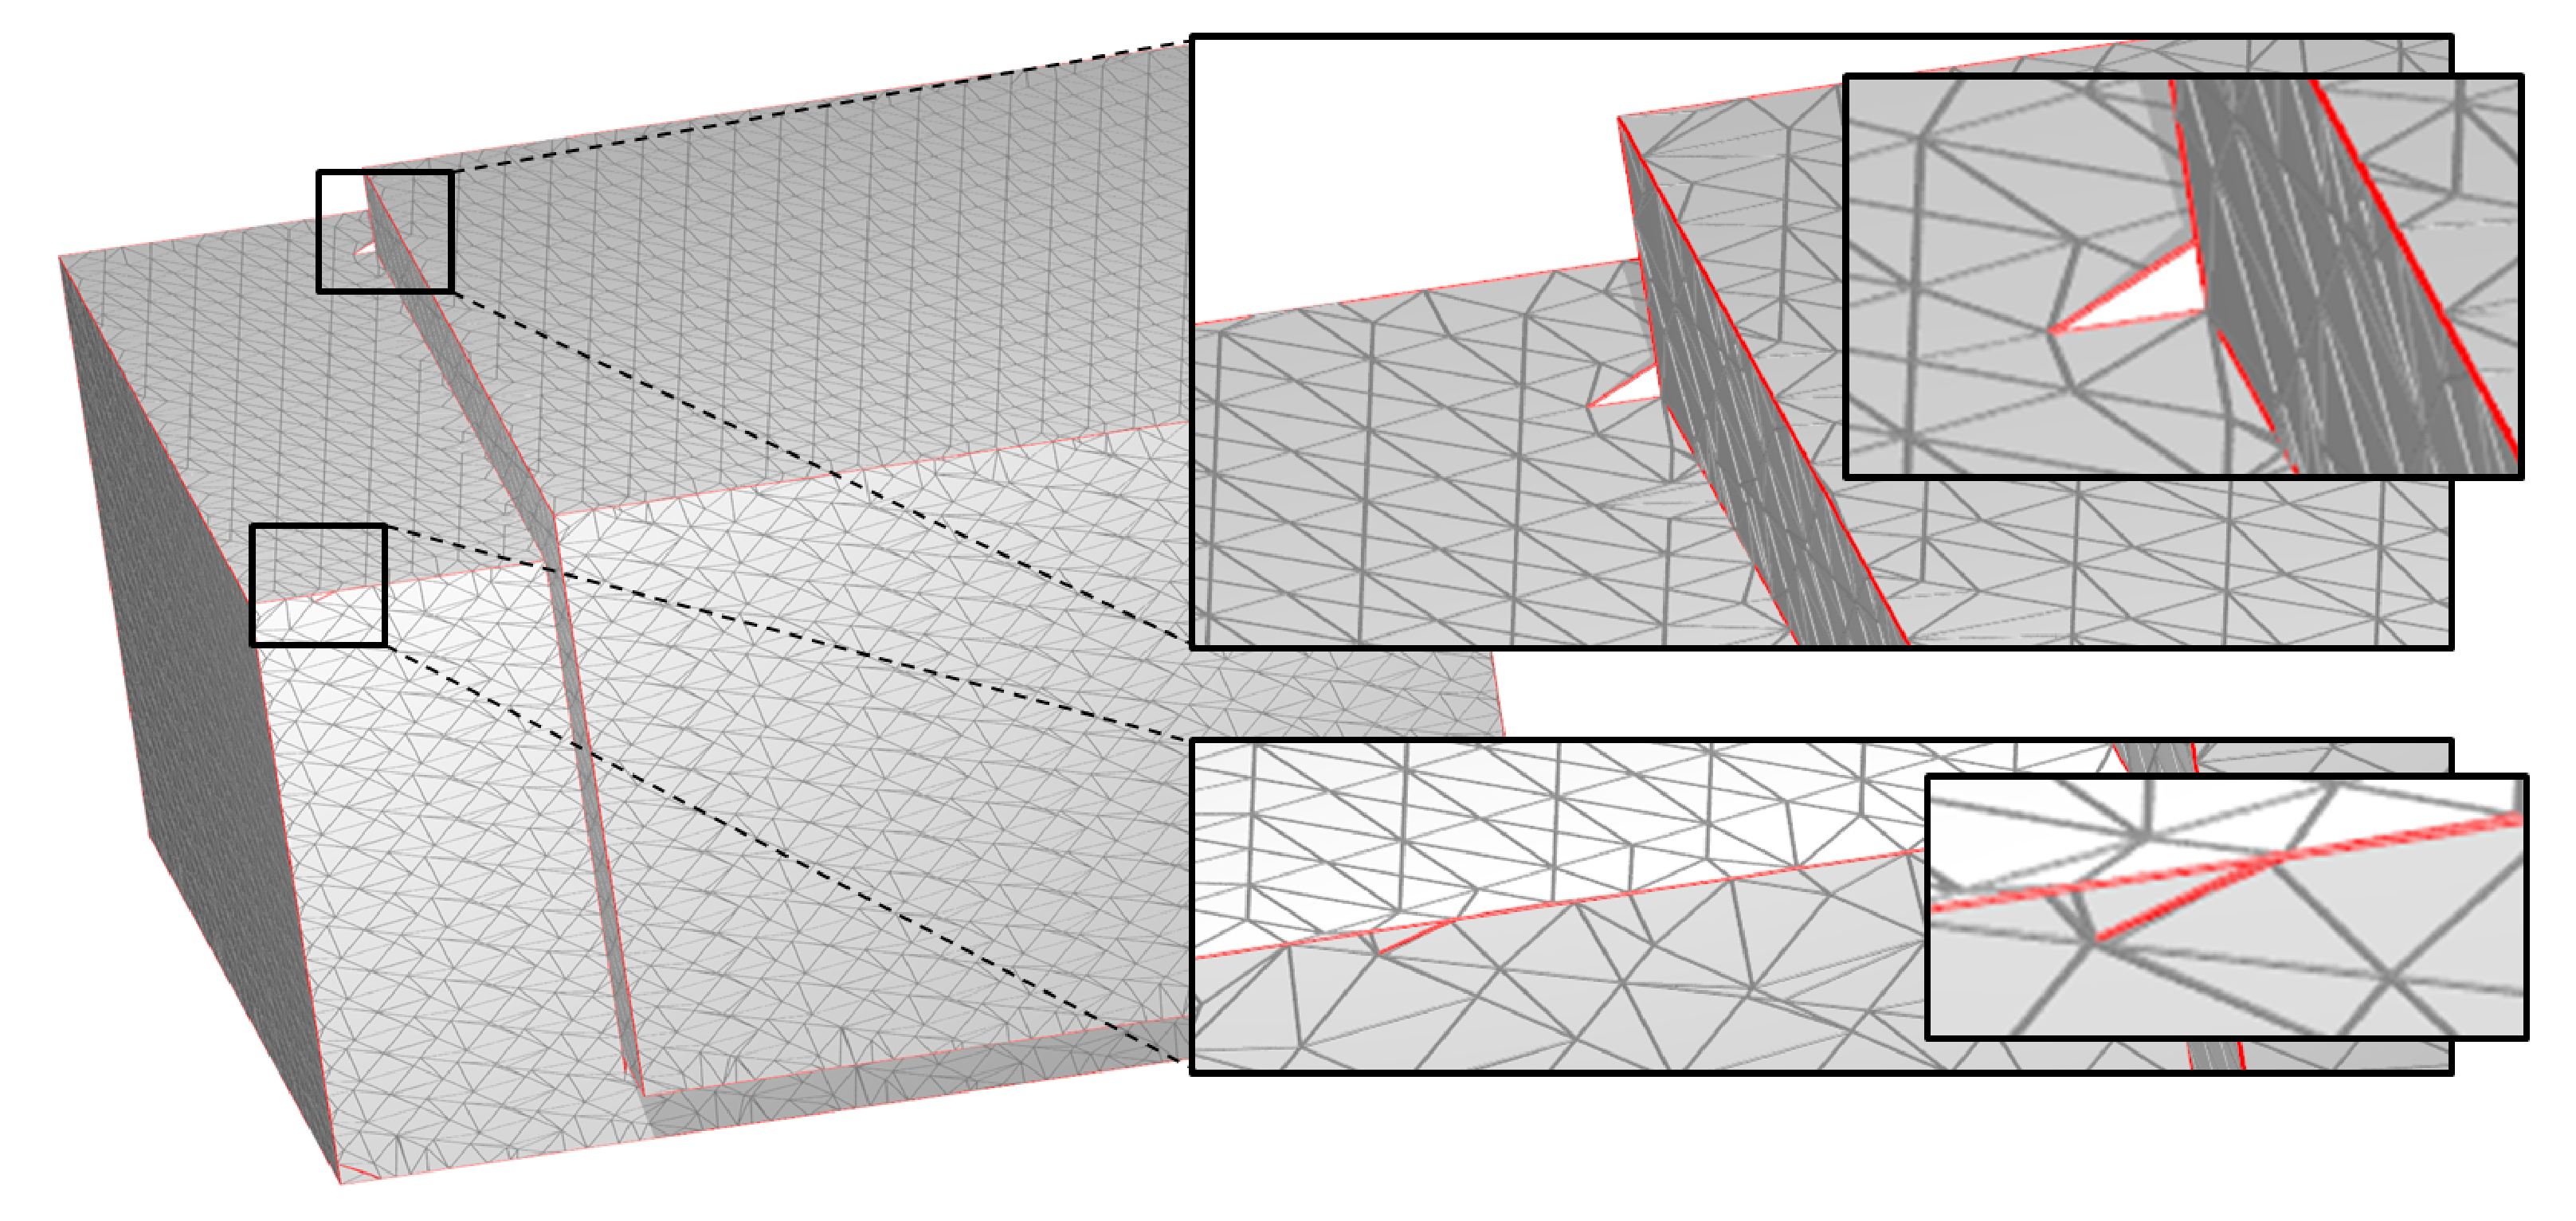
\includegraphics[width=0.7\linewidth]{images/isoExTwoCube.eps}\label{fig:isoEx:b}}
	\caption{Extended Marching Cubes results. (a) Extended Marching Cubes on a Flange dataset. (b) Extended Marching Cubes on a TwoCube dataset.}	
\end{figure}
We also compare our algorithm to Extended Marching Cubes by Kobbelt et al.~\cite{kbsh-fssev-01}. Figure~\protect\subref*{fig:isoEx:a},~\protect\subref*{fig:isoEx:b} shows the results of running Extended Marching Cubes on a Flange and a TwoCube dataset respectively. The magnified regions show that Extended Marching Cubes (same as Marching Cubes) is prone to producing small triangles. Occasionally Extended Marching Cubes also produces creases. 
\subsection{Timings}

